%\let\proof\relax
%\let\endproof\relax

\documentclass[final,12pt]{colt2018} % Anonymized submission
% \documentclass{colt2017} % Include author names

% The following packages will be automatically loaded:
% amsmath, amssymb, natbib, graphicx, url, algorithm2e

\title[Non-Convex Matrix Completion Against a Semi-Random Adversary]{Non-Convex Matrix Completion Against a Semi-Random Adversary}
\usepackage{times}
 % Use \Name{Author Name} to specify the name.
 % If the surname contains spaces, enclose the surname
 % in braces, e.g. \Name{John {Smith Jones}} similarly
 % if the name has a "von" part, e.g \Name{Jane {de Winter}}.
 % If the first letter in the forenames is a diacritic
 % enclose the diacritic in braces, e.g. \Name{{\'E}louise Smith}

 % Two authors with the same address
 \coltauthor{\Name{Yu Cheng} \Email{yucheng@cs.duke.edu}\AND
  \Name{Rong Ge} \Email{rongge@cs.duke.edu}\\
  \addr Duke University}

 % Three or more authors with the same address:
 % \coltauthor{\Name{Author Name1} \Email{an1@sample.com}\\
 %  \Name{Author Name2} \Email{an2@sample.com}\\
 %  \Name{Author Name3} \Email{an3@sample.com}\\
 %  \addr Address}
 
 % Authors with different addresses:
% \coltauthor{\Name{Author Name1} \Email{abc@sample.com}\\
% \addr Address 1
% \AND
% \Name{Author Name2} \Email{xyz@sample.com}\\
% \addr Address 2
% }


%\usepackage{amsmath,amsfonts,amsthm,amssymb,color}

%\usepackage{fullpage}

%\newtheorem{theorem}{Theorem}[section]
%\newtheorem{corollary}[theorem]{Corollary}
%\newtheorem{lemma}[theorem]{Lemma}
%\newtheorem{observation}[theorem]{Observation}
%\newtheorem{proposition}[theorem]{Proposition}
%\newtheorem{conjecture}[theorem]{Conjecture}
%\newtheorem{claim}[theorem]{Claim}
%\newtheorem{fact}[theorem]{Fact}
%\newtheorem{assumption}[theorem]{Assumption}
%\theoremstyle{definition}
%\newtheorem{definition}[theorem]{Definition}
\newtheorem{problem}{Problem}
%\newtheorem{remark}[theorem]{Remark}

% Color edits
%\usepackage{color-edits}
%\usepackage[suppress]{color-edits}  % to get rid of all color

%\addauthor[Rong]{rg}{blue}
%\addauthor[Yu]{yc}{red}

% We now have the macros:
% - \ycedit{text}: prints text in red
% - \yccomment{text}: prints [Yu: text] in red
% - \ycmargincomment{text}: prints [Yu: text] in red in the margin
% - \ycdelete{text}: marks in the margin in red that Yu deleted here

% Yu
%\usepackage{hyperref}
%\usepackage[ruled,vlined]{algorithm2e}
%\usepackage{graphicx}
\usepackage{xspace}
\usepackage{ifthen}
%\usepackage{color}
%\newcommand{\todo}[1]{{\color{red} TODO: #1}}

\newcommand{\eps}{\ensuremath{\epsilon}\xspace}
\renewcommand{\tilde}{\widetilde}
\renewcommand{\hat}{\widehat}
\renewcommand{\bar}{\overline}
\newcommand{\eqdef}{:=}
%\newcommand{\eqdef}{\ensuremath{\overset{\mathrm{def}}{=}}\xspace}
\newcommand{\R}{\mathbb{R}}
\newcommand{\C}{\mathbb{R}}
\newcommand{\OO}{\mathcal{O}}

\DeclareMathOperator{\tr}{tr}
\newcommand{\norm}[1]{\lVert#1{\rVert}}
\newcommand{\normone}[1]{{\norm{#1}}_1}
\newcommand{\normtwo}[1]{{\norm{#1}}_2}
\newcommand{\norminf}[1]{{\norm{#1}}_\infty}
\newcommand{\fnorm}[1]{{\norm{#1}}_F}
\newcommand{\maxnorm}[1]{{\norm{#1}}_{\max}}
\providecommand{\expect}[2]{\ensuremath{\ifthenelse{\equal{#1}{}}{\mathbb{E}}{\mathbb{E}_{#1}}\left[#2\right]}\xspace}

% LP environment
\newcommand{\mini}[1]{\mbox{minimize} & {#1} &\\}
\newcommand{\maxi}[1]{\mbox{maximize} & {#1 } & \\}
\newcommand{\st}{\mbox{subject to} }
\newcommand{\con}[1]{&#1 & \\}
\newcommand{\qcon}[2]{&#1, & \mbox{for } #2.  \\}
\newenvironment{lp}{\begin{equation}  \begin{array}{lll}}{\end{array}\end{equation}}
\newenvironment{lp*}{\begin{equation*}  \begin{array}{lll}}{\end{array}\end{equation*}}

% Rong
\newcommand{\nnz}{\text{nnz}\xspace}
\newcommand{\inner}[1]{\langle #1\rangle}
\newcommand{\Us}{U^\star}
\newcommand{\Vs}{V^\star}
\newcommand{\Ms}{M^\star}
\newcommand{\Sigs}{\Sigma^\star}
\newcommand{\sigs}{\sigma^\star}


\begin{document}

%\title{Non-Convex Matrix Completion Against a Semi-Random Adversary}
%\author{Yu Cheng \qquad Rong Ge \\ Duke University}
%\date{}

\maketitle

We present preconditioned stochastic gradient descent (SGD) algorithms for the $\ell_1$ minimization problem $\min_{\xx}\|\AA \xx - \bb\|_1$ in the overdetermined case, where there are far more constraints than variables. Specifically, we have $\AA \in \R^{n \times d}$ for $n \gg d$. Commonly known as the Least Absolute Deviations problem, $\ell_1$ regression can be used to solve many important combinatorial problems, such as minimum cut and shortest path. SGD-based algorithms are appealing for their simplicity and practical efficiency.
% Our algorithms precondition the matrix $\AA$ and then solve the problem for the resulting matrix $\tilde{\AA}$ using gradient descent techniques.
Our primary insight is that careful preprocessing can yield preconditioned matrices $\tilde{\AA}$ with strong properties (besides good condition number and low-dimension) that allow for faster convergence of gradient descent. In particular, we precondition using Lewis weights to obtain an isotropic matrix with fewer rows and strong upper bounds on all row norms. We leverage these conditions to find a good initialization, which we use along with recent smoothing reductions and accelerated stochastic gradient descent algorithms to achieve $\epsilon$ relative error in $\Otil(nnz(\AA) + d^{2.5} \epsilon^{-2})$ time with high probability, where $nnz(\AA)$ is the number of non-zeros in $\AA$. This improves over the previous best result using gradient descent for $\ell_1$ regression. We also match the best known running times for interior point methods in several settings.

Finally, we also show that if our original matrix $\AA$ is approximately isotropic and the row norms are approximately equal, we can give an algorithm that avoids using fast matrix multiplication and obtains a running time of $\Otil(nnz(\AA) + s d^{1.5}\epsilon^{-2} + d^2\epsilon^{-2})$, where $s$ is the maximum number of non-zeros in a row of $\AA$. In this setting, we beat the best interior point methods for certain parameter regimes.


%We consider the $\ell_1$ minimization problem $\min_{\xx}||\AA \xx - \bb||_1$ in the overconstrained case, where there are far more constraints than variables. More specifically, we have $\AA \in \R^{n \times d}$ for $n \gg d$. By using Lewis Weights preconditioning on $\AA$ and a careful initialization, we show that a standard stochastic gradient descent algorithm achieves $\epsilon$ relative error in about $nnz(\AA) +  d^3\epsilon^{-2}$ time with high probability. If we leverage smoothing reductions in \cite{AllenZhuH16} and the accelerated stochastic gradient descent algorithms in \cite{AllenZhu17}, we can achieve a running time of about $nnz(\AA) + d^{2.5}\epsilon^{-2}$ with the same guarantees. Both of these running times improve over the previous results in \cite{YangCRM16} and the latter result is comparable to the best known running times for interior point methods \cite{LeeS15}.
%
%The key idea will be to use our preconditioning to restrict our consideration to matrices $\AA$ such that $\AA^T\AA = \II$ and every row norm of $\AA$ is upper bounded by $O(\sqrt{d/n})$. \cite{cohenpeng} show that sampling $\AA$ with Lewis weights takes about $nnz(\AA) +d^{\omega}$ time and approximately preserves the minimization problem. Moreover, we can assume $n\le O(d\epsilon^{-2}\log n)$ for the sampled matrix. We then prove that all leverage scores of the sampled matrix are approximately equal. Since rotations preserve leverage scores, we can then rotate our sampled matrix to ensure that our desired properties are met in about $d^{\omega}\epsilon^{-2}$ time.
%
%Finally, we also show that if our original matrix $\AA$ is such that $\AA^T\AA \approx \II$ and the row norms of $\AA$ are bounded, we can avoid using fast matrix multiplication and prove a running time of about $nnz(\AA) + s d^{1.5}\epsilon^{-2}$, where $s$ is the maximum number of non-zeros in a row of $\AA$.

%Consequently, we will be able to restrict our consideration to matrices $A$ such that $A^TA \approx I$, and all row norms are equal, which is to say $||A_{i,:}||_2 = \sqrt{\frac{d}{n}}$ for all $i$.
%
%With a careful choice of our initial $x$, we show that standard gradient descent and stochastic gradient descent algorithms under these further assumptions only require $O(\frac{d}{\epsilon^2})$ and $O(\frac{d^2}{\epsilon^2})$ iterations, respectively, to achieve $\epsilon$ relative error with respect to the minimum objective value. Accordingly, these methods each achieve respective total runtime of $O(\frac{md}{\epsilon^2})$ and $O(\frac{d^3}{\epsilon^2})$, along with an $O(m)$ preconditioning cost, improving over the previous results in \cite{MahoneySGD}.
%
%We further examine the consequences of our assumptions when combined with smoothing reductions in [cite] and accelerated gradient descent techniques in [cite,cite]. As a result we are able to further improve the running times to $O(\frac{md}{\epsilon})$ and $O(dn\log{1/\epsilon} + \frac{d^2\sqrt{n}}{\epsilon})$.
%
%Random sampling $d\epsilon^{-2}\log{d}$ rows of $A$ will only incur error $\epsilon$ and reduces the latter running time to $O(\frac{d^{2.5}\log{d}}{\epsilon^2})$, which is then comparable to interior point methods of [cite]


%\pagenumbering{gobble}
%\newpage
%\pagenumbering{arabic}

\begin{keywords}
Matrix Completion, Non-Convex Optimization, Semi-Random Model.
\end{keywords}



% !TeX root = main.tex
\section{Introduction}
\label{sec:intro}
Generative models are often trained in an unsupervised fashion, fitting a model $q$ to a set of observed data $x_P \subseteq X$ drawn iid from some true distribution $p$ on $x\in X$. Now, of course $p$ may not exactly belong to family $Q$ of probability distributions being fit, whether $Q$ consists of Gaussians mixture models, Markov models, or even neural networks of bounded size. We first discuss the limitations of generative modeling without feedback, and then discuss our model and results.

%\subsection{Limitations of Generative Modeling from Positive Examples Alone}
Consider fitting a generative model on a text corpus consisting partly of poetry written by four-year-olds and partly of mathematical publications from the {\em Annals of Mathematics}. Suppose that learning to generate a poem that looks like it was written by a child was easier than learning to generate a novel mathematical article with a correct, nontrivial statement. If the generative model pays a high price for generating unrealistic examples, then it may be better off learning to generate children's poetry than mathematical publications. However, without negative feedback, it may be difficult for a neural network or any other model to know that the mathematical articles it is generating are stylistically similar to the mathematical publications but do not contain valid proofs.\footnote{This is excluding clearly fake articles published without proper review in lower-tier venues \citep{LabbeL13}.} 

As a simpler example, the classic Markovian ``trigram model'' of natural language assigns each word a fixed probability conditioned only on the previous two words. Prior to recent advances in deep learning, for decades the trigram model and its variant were the workhorses of language modeling, assigning much greater likelihood to natural language corpora than numerous linguistically motivated grammars and other attempts \citep{Rosenfeld00}. However, text sampled from a trigram is typically nonsensical, e.g., the following text was randomly generated from a trigram model fit on a corpus of text from the Wall Street Journal \citep{JurafskyM09}:
\begin{quote}
They also point to ninety nine point six billion dollars from two hundred
four oh six three percent of the rates of interest stores as Mexico and
gram Brazil on market conditions. 
\end{quote}

In some applications, like text compression using a language model \citep{WittenNC87}, maximizing likelihood is equivalent to optimizing compression. However, in many  applications involving generation, such nonsense is costly and unacceptable. Now, of course it is possible to always generate valid data by returning random training examples, but this is simply overfitting and not learning. Alternatively, one could incorporate human-in-the-loop feedback such as through crowdsourcing, into the generative model to determine what is a valid, plausible sentence.

In some domains, validity could be determined automatically. Consider a Markovian model of a well-defined concept such as mathematical formulas that compile in \LaTeX{}. Now, consider a $n$-gram Markovian character model which the probability of each subsequent character is determined by the previous $n$ characters. For instance, the expression \$\{2+\{x-y\}\$ is invalid in \LaTeX{} due to mismatched braces. For this problem, a \LaTeX{} compiler may serve as a validity oracle. Various $n$-gram models can be fit which only generate valid formulas. To address mismatched braces, for example, one such model would ensure that it always closed braces within $n$ characters of opening, and had no nested braces. While an $n$-gram model will not perfectly model the true distribution over valid \LaTeX{} formulas, for certain generative purposes one may prefer an $n$-gram model that generates valid formulas over one that assigns greater likelihood to the training data but generates invalid formulas. 

Figure \ref{fig:rectangle} illustrates a simple case of learning a rectangle model for data which is not uniform over a rectangle. A maximum likelihood model would necessarily be the smallest rectangle containing all the data, but most examples generated from this distribution may be invalid. Instead a smaller rectangle, as illustrated in the figure, may be desired.

\begin{figure}[h]\label{fig:rectangle}
\centering
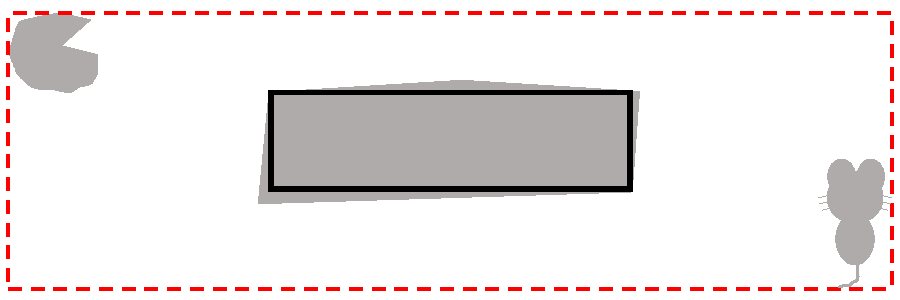
\includegraphics[width=3in]{fig.pdf}
\caption{Example where the underlying distribution $p$ is uniform over the (gray) valid regions. The solid rectangle maximizes our objective since it does not output nonsense (is supported only within the grey matter) and is closest to the $p$ (covers the maximum amount of grey matter). In contrast, the standard maximum likelihood (dashed red) rectangle must fully contain the observed samples, thus generating invalid points most of the time.  }
\end{figure}

Motivated by these observations, we evaluate a generative model $q$ on two axes. First is {\em coverage}, which is related to the probability assigned to future examples drawn from the true distribution $p$. Second is {\em validity}, defined as the probability that random examples generated from $q$ meet some validity requirement. Formally, we measure coverage in terms of a bounded {\em loss}:
$$\Loss(p,q)=\E_{x \sim p}[L(q_x)],$$
where $L:[0,1]\rightarrow [0,M]$ is a bounded decreasing function such as the capped log-loss $L(q_x)=\min(M, \log 1/q_x)$. % or $L(q_x)=\log 1/(q_x+\exp(-M))$. 
A bounded loss has the advantages of being efficiently estimable, and also it enables a model to assign 0 probability to one example (e.g., an outlier or error) if it greatly increases the likelihood of all other data. Validity is defined with respect to a set $V \subseteq X$, and $q(V)$ is the probability that a random example generated from $q$ lies within $V$. 

Clearly, there is a tradeoff between coverage and validity. We first focus on the case of (near) perfect validity. A Valid Generative Modeling (VGM) algorithm if it outputs, for a family of distributions $Q$ over $X$, if it outputs $\hat{q}$ with (nearly) perfect validity and whose loss is nearly as good as the loss of the best valid $q\in Q$. More precisely, $A$ is a VGM learner of $Q$ if for any nonempty valid subset $V \subseteq X$, any probability distribution $p$ over $V$, and any $\eps>0$, $A$ uses $n$ random samples from $p$ and makes $m$ membership oracle calls to $V$ and outputs a distribution $\hat{q}$ such that, $$\Loss(p, \hat{q}) \leq \min_{q \in Q: q(V)=1}\Loss(p,q) + \eps ~\text{ and }~\hat{q}(V)\geq 1-\eps.$$ 
We aim for our learner to be sample and query efficient, requiring that $n$ and $m$ are polynomial in $M, 1/\eps$ and a measure of complexity of our distribution class $Q$.
Furthermore, we would like our algorithms to be computationally efficient, with a runtime polynomial in the size of the data, namely the $n + m$ training examples. 
A more formal description of the problem is available in Section~\ref{sec:problem}.

$A$ is said to be {\em proper} if it always outputs $\hat{q}\in Q$ and {\em improper} otherwise.
In Section~\ref{sec:impossibility}, we first show that efficient proper learning for VGM is impossible. This is an information-theoretic result, meaning that even given infinite runtime and positive samples, one still cannot solve the VGM problem. Interestingly, this is different from binary classification, where it is possible to statistically learn from iid examples without a membership oracle.

Our first main positive result is an efficient (improper) learner for VGM. The algorithm relies on a subroutine that solves the following {\em Generative Modeling with Negatives} (GMN) problem: given sets $X_P, X_N \subset X$ of positive and negative examples, find the probability distribution $q \in Q$ which minimizes $\sum_{x \in X_P} L(q(x))$ subject to the constraint that $q(X_N)=0$. For simplicity, we present our algorithm for the case that the distribution family $Q$ is finite, giving sample and query complexity bounds that are logarithmic in terms of $|Q|$. However, as we show in Section~\ref{sec:infinite-families}, all of our results extend to infinite families $Q$. It follows that if one has a computationally efficient algorithm for the GMN problem for a distribution family $Q$, then our reduction gives a computationally efficient VGM learning algorithm for $Q$.

Our second positive result is an algorithm that minimizes $\Loss(p,q)$ subject to a relaxed validity constraint comparing against the optimal distribution that has validity $q(V)$ at least $1-\alpha$ for some $\alpha>0$. We show in Section~\ref{sec:partial-validity} that even in this more general setting, it is possible to obtain an algorithm that is statistically efficient but may not be computationally efficient. An important open question is whether there exists a computationally efficient algorithm for this problem when given access to an optimization oracle, as was the case for our algorithm for VGM.

\subsection{Related Work}
\cite{KearnsMRRSS94} showed how to learn distributions from positive examples in the realizable setting, i.e., where the true distribution is assumed to belong to the class being learned. In the same sense as their work is similar to PAC learning \citet{Valiant84} of distributions, our work is like agnostic learning \citet{KearnsSS94} in which no assumption on the true distribution is made. 

Generative Adversarial Networks (GANs)~\cite{GoodfellowPMXWOCB14} are an approach for generative modeling from positive examples alone, in which a generative model is trained against a discriminator that aims to distinguish real data from generated data. In some domains, GANs have been shown to outperform other methods at generating realistic-looking examples. Several shortcomings of GANs have been observed \citet{AroraRZ18}, and GANs are still subject to the theoretical limitations we argue are inherent to any model trained without a validity oracle. 

In supervised learning, there is a rich history of learning theory with various types of queries, including membership which are not unlike our (in)validity oracle. Under various assumptions, queries have been shown to facilitate the learning of complex classes such as finite automata \citet{Angluin88} and DNFs \citet{Jackson97}. See the survey of \cite{Angluin92} for further details.  Interestingly, \cite{Feldman09} has shown that for agnostic learning, i.e., without making assumptions on the generating distribution, the addition of membership queries does not enhance what is learnable beyond random examples alone. 
Supervised learning also has a large literature around active learning, showing how the ability to query examples reduces the sample complexity of many algorithms. See the survey of \cite{Hanneke14}. Note that the aim here is typically to save examples and not to expand what is learnable.
 
More sophisticated models, e.g., involving neural networks, can mitigate the invalidity problem as they often generate more realistic natural language and have even been demonstrated to generate \LaTeX{} that nearly compiles \citep{Karpathy15} or nearly valid Wikipedia markdown. However, longer strings generated are unlikely to be valid. For example, \cite{Karpathy15} shows generated markdown which includes:
\begin{quote}
==Access to ''rap===
The current history of the BGA has been [[Vatican Oriolean Diet]], British Armenian, published in 1893.  While actualistic such conditions such as the [[Style Mark Romanians]] are still nearly not the loss.
\end{quote}

Even ignoring the mismatched quotes and equal signs, note that this example has two so-called ``red links'' to two pages that do not exist. Without checking, it was not obvious to us whether or not Wikipedia had pages titled {\em Vatican Oriolean Diet} or {\em Style Mark Romanians}. In some applications, one may or may not want to disallow red links. In the case that they are considered valid, one may seek a full generative model of what might plausibly occur inside of brackets, as the neural network has learned in this case. If they are disallowed, a model might memorize links it has seen but not generate new ones. A validity oracle can help the learner identify what it should avoid generating.

 In practice, \cite{KusnerPH17} discuss how generative models from neural networks (in particular autoencoders) often generate invalid sequences. 
\cite{JanzWPKH18} learn the validity of examples output by a generative model using oracle feedback. 


%!TEX root = main.tex

\section{Preliminaries}
In this section, we will review some well-known results on~\gd~and~\nag~in the strongly convex setting, 
and existing results on convergence of~\gd~to second-order stationary points. 
% The pseudocode for these algorithms is given in Algorithms~\ref{algo:gd} and~\ref{algo:AGD} respectively.

% \cnote{Show gradient descent in equation}

\subsection{Notation}
Bold upper-case letters ($\A, \B$) denote matrices and bold lower-case letters ($\x, \y$) denote vectors. 
For vectors $\norm{\cdot}$ denotes the $\ell_2$-norm. For matrices, $\norm{\cdot}$ denotes the spectral norm and $\lambda_{\min}(\cdot)$ denotes the minimum eigenvalue.
For $f: \R^d \rightarrow \R$, $\grad f(\cdot)$ and  $\hess f(\cdot)$ denote its gradient and Hessian respectively, and $f^\star$ denotes its global minimum.
% Other than Section \ref{sec:related}, 
We use $O(\cdot), \Theta(\cdot), \Omega(\cdot)$ to hide absolute constants, and $\tilde{O}(\cdot), \tilde{\Theta}(\cdot), \tilde{\Omega}(\cdot)$ to hide absolute constants and polylog factors for all problem parameters. 
% \praneeth{I think it will be cleaner to make the dependence on smoothness parameters in Table~\ref{tab:main} and edit this statement} \jccomment{Then I also need to add function value dependence, maybe too complicated to compare}.\praneeth{The issue with this is that $O()$ is not just hiding constants but also problem dependent parameters. May be mention this explicitly in the caption to the table.} 
% We let $\ball^{(d)}_\x(r)$ denote the d-dimensional ball centered at $\x$ with radius $r$; when it is clear from context, we simply denote it as $\ball_\x(r)$. We use $\proj_{\mathcal{X}}(\cdot)$ to denote projection onto the set $\mathcal{X}$. Distance and projection are always defined in a Euclidean sense.


% \pn{Talk about ignoring $\log d$ factors in notation.}

\subsection{Convex Setting}\label{sec:prelim_convex}
% \begin{figure}[t]
% \begin{minipage}{0.5\textwidth}
% 	\begin{algorithm}[H]
% 	\caption{\gd($\x_0, \eta$)}\label{algo:gd}
% 	\begin{algorithmic}[1]
% 		\For{$t = 0, 1, \ldots, T $}
% 		\State $\x_{t+1} \leftarrow \x_t - \eta \grad f (\x_t)$
% 		\EndFor
% 		\State \textbf{return} $\x_T$
% 	\end{algorithmic}
% 	\end{algorithm}
% 	\vspace{0.5cm}
% \end{minipage}
% \begin{minipage}{.5\textwidth}

% \end{minipage}
% \end{figure}
To minimize a function $f(\cdot)$,~\gd ~performs the following sequence of steps:
\begin{equation*}
\x_{t+1} = \x_{t}- \eta \grad f(\x_t).
\end{equation*}
The suboptimality of~\gd~and the improvement achieved by~\nag~can be clearly illustrated for the case of smooth and strongly convex functions. %The definitions of smoothness and strong convexity are as follows.
\begin{definition}\label{def:smooth}
A differentiable function $f(\cdot)$ is \textbf{$\ell$-smooth (or $\ell$-gradient Lipschitz)} if:
\begin{equation*}
\norm{\grad f(\x_1) - \grad f(\x_2)} \le \ell \norm{\x_1 - \x_2} \quad \forall \; \x_1, \x_2.
\end{equation*}
\end{definition}
\noindent
The gradient Lipschitz property asserts that the gradient can not change too rapidly in a small local region.
\begin{definition}\label{def:convex}
A twice-differentiable function $f(\cdot)$ is \textbf{$\alpha$-strongly convex} if
$\lambda_{\min}(\hess f(\x)) \ge \alpha, \;  \forall \; \x$.
% $f(\x_2) \ge f(\x_1) + \la \grad f(\x_1), \x_2 - \x_1 \ra + \frac{\alpha}{2}\norm{\x_2 - \x_1}^2, \quad \forall \; \x_1, \x_2.$
\end{definition}
Let $\fstar \defeq \min_{\y}f(\y)$. A point $\x$ is said to be \textbf{$\epsilon$-suboptimal} if $f(\x)  \le  \fstar + \epsilon$. The following theorem gives the convergence rate of GD and AGD for smooth and strongly convex functions.
\begin{theorem}[\cite{nesterov2004introductory}]\label{thm:gd_convex}
Assume that the function $f(\cdot)$ is $\ell$-smooth and $\alpha$-strongly convex. Then, for any $\epsilon>0$,
the iteration complexities to find an $\epsilon$-suboptimal point are as follows:
\begin{itemize}
\item GD with $\eta  = 1/\ell$: \quad $O((\ell/\alpha) \cdot \log ((f(\x_0) - \fstar)/\epsilon))$
\item AGD (Algorithm~\ref{algo:AGD}) with $\eta = 1/\ell$ and $\theta = \sqrt{\alpha/\ell}$:
\quad$O(\sqrt{\ell/\alpha} \cdot \log ((f(\x_0) - \fstar)/\epsilon))$.
\end{itemize}
% ~\gd~with $\eta = \frac{1}{\ell}$ will output an \ESP ~in iterations:
% \begin{equation*}
% O\left(\frac{\ell}{\alpha}\log \frac{f(\x_0) - \fstar}{\epsilon}\right).
% \end{equation*}
\end{theorem}

The number of iterations of GD depends linearly on the ratio $\ell/\alpha$, which is called the condition number of $f(\cdot)$ since $\alpha \I \preceq\hess f(\x) \preceq \ell \I $. Clearly $\ell \geq \alpha$ and hence condition number is always at least one. Denoting the condition number by ${\cn}$, we highlight two important aspects of~\nag: (1) the momentum parameter satisfies $\theta = 1/\sqrt{\cn}$ and (2) \nag~improves upon GD by a factor of $\sqrt{\cn}$. 
% The following theorem gives the convergence rate of~\nag~for these problems.
% \begin{theorem}[\cite{nesterov2004introductory}]\label{thm:agd_convex}
% Assume that the function $f(\cdot)$ is $\ell$-smooth and convex. Then, for any $\epsilon>0$,~\nag~with $\eta = \frac{1}{\ell}$ and $\theta = \Theta(\sqrt{\frac{\alpha}{\ell}}) $ will output an~\ESP~in iterations:
% \begin{equation*}
% O\left(\sqrt{\frac{\ell}{\alpha}}\log \frac{f(\x_0)-\fstar }{\epsilon}\right).
% \end{equation*}
% \end{theorem}
% \noindent
% Note that the rate here improves upon that of~\gd~by a factor of $\sqrt{\frac{\ell}{\alpha}}$ i.e., squareroot of the condition number.
%say something about condition number.

\subsection{Nonconvex Setting}
For nonconvex functions finding global minima is NP-hard in the worst case. The best one can hope for in this setting is convergence to stationary points. There are various levels of stationarity.
\begin{definition}
$\x$ is an \textbf{\EFSP} of function $f(\cdot)$ if $\norm{\grad f(\x)} \le \epsilon$.
\end{definition}
\noindent
As mentioned in Section~\ref{sec:intro}, for most nonconvex problems encountered in practice, a majority of first-order stationary points turn out to be saddle points. Second-order stationary points require not only zero gradient, but also positive semidefinite Hessian, ruling out most saddle points.
%Therefore, this paper focus on finding second-order stationary point.
%In order to discuss Hessian-related properties meaningfully, we first need to assert Hessian smoothness condition.
Second-order stationary points are meaningful, however, only when the Hessian is continuous.
% second order stationary points which means that in addition to being first order stationary points, the Hessian at these points is almost positive semidefinite. This is meaningful only if the Hessian does not change arbitrarily (and perhaps have large negative eigenvalues) in a small neighborhood around this point. In other words, finding second order stationary points is meaningful only if the Hessian is continuous.
%\cnote{Should we talk the case where gradient is Lipschitz but Hessian is not?}
% \begin{theorem}[\citep{nesterov1998introductory}]\label{thm:grad_smooth}
% Assume that the function $f(\cdot)$ is $\ell$-smooth. Then, for any $\epsilon>0$, gradient descent will output an \EFSP ~in iterations:
% \begin{equation*}
% \frac{\ell(f(\x_0) - f^\star)}{\epsilon^2}.
% \end{equation*}
% \end{theorem}
\begin{definition}\label{def:HessianLip}
A twice-differentiable function $f(\cdot)$ is \textbf{$\rho$-Hessian Lipschitz} if:
\begin{equation*}
\norm{\hess f(\x_1) - \hess f(\x_2)} \le \rho \norm{\x_1 - \x_2} \quad \forall \; \x_1, \x_2.
\end{equation*}
\end{definition}
%\noindent
% For Hessian Lipschitz functions, we recall the definition of second order stationary points from~\cite{nesterov2006cubic}.
\begin{definition}[\cite{nesterov2006cubic}]\label{def:SOSP}
For a $\rho$-Hessian Lipschitz function $f(\cdot)$, $\x$ is an \textbf{\ESSP} if:
% $\norm{\grad f(\x)} \le \epsilon$ and $\lambda_{\min}(\hess f(\x)) \ge - \sqrt{\rho \epsilon}$.
\begin{equation*}
\norm{\grad f(\x)} \le \epsilon \quad\text{and}\quad \lambda_{\min}(\hess f(\x)) \ge - \sqrt{\rho \epsilon}.
\end{equation*}
\end{definition}
\noindent
The following theorem gives convergence rate of perturbed~\gd~to second-order stationary points.
%See~\cite{jin2017escape} for a detailed description of the algorithm.
\begin{theorem}[\citep{jin2017escape}]\label{thm:perturbed_GD}
Assume that the function $f(\cdot)$ is $\ell$-smooth and $\rho$-Hessian Lipschitz. Then, for any $\epsilon>0$, perturbed GD outputs an \ESSP ~w.h.p in iterations:
\begin{equation*}
\otilde{\frac{\ell(f(\x_0) - \fstar)}{\epsilon^2}}.
\end{equation*}
\end{theorem}
\noindent
Note that this rate is essentially the same as that of~\gd~for convergence to first-order stationary points. In particular, it only has polylogarithmic dependence on the dimension.


% !TEX root = main.tex

\section{Pre-Processing: Reweighting the Entries}
\label{sec:bss}

In this section, we present a nearly-linear time algorithm for Problem~\ref{prob:main}.
As we discussed in Section~\ref{sec:laplacian}, Problem~\ref{prob:main} is equivalent to the problem of approximating the identity matrix (Problem~\ref{prob:identity}). We prove the following theorem for Problem~\ref{prob:identity}:

\begin{theorem}[Our Preprocessing Algorithm]
\label{thm:bss}
Fix $0 \le \eps, \beta \le 1/10$, and a graph Laplacian $L \in \R^{n \times n}$.
Given a set of $m$ vectors $\{v_i\}_{i=1}^m$, where each $v_i = L^{-1/2} b_i$ for some $b_i$ representing an edge (with only two non-zero entries, one $+1$ and one $-1$).
Assume there exist weights $w_i \ge 0$ such that~\footnote{We assume $0<\beta\le\frac{1}{10}$ is given, because we can do a binary search by running our algorithm and see if it succeeds.
It is worth mentioning that we never explicitly compute any $v_i = L^{-1/2} b_i$. %We will maintain a set of weights $\{\tilde w_i\}$ which will eventually satisfy the claim.
See Appendix~\ref{app:bss} for more details.}
\[
\textstyle (1-\beta) I \preceq \sum_{i=1}^m w_i v_i v_i^\top \preceq (1+\beta) I.
\]
We can find a set of weights $\tilde w_i \ge 0$ in $\tilde O(m / \eps^{O(1)})$ time, such that with high probability,
\[
\textstyle (1-O(\beta)-\eps)I \preceq \sum_{i=1}^m \tilde w_i v_i v_i^\top \preceq I.
\]
\end{theorem}

%In other words, we can solve the following class of SDP approximately in nearly linear time.
%\begin{lp}
%\mini{\normtwo{I - \sum_{i=1}^m w_i v_i v_i^\top}}
%\st \con{w_i \ge 0}
%\end{lp}
We adapt techniques from recent developments on linear-sized graph sparsification~\citep{BatsonSS12, AllenLO15, LeeS17}.
The main difference between our problem and the graph sparsification problem is the following: instead of assuming $\sum_i v_i v_i^\top = I$, we only know the \emph{existence} of an unknown set $S$ such that \mbox{$\sum_{i\in S} v_i v_i^\top = I$}.
%In other words, the graph that we are trying to approximate (e.g., the complete bipartite graph) has spectral properties different from the input graph.
This prevents us from using some of the well-known techniques in graph sparsification (e.g., sampling by effective resistance \cite{SpielmanS11, LeeS15}).
%In other words, our goal is to find a set of weights $\{w_i\}_i$ so that $\sum_i w_i v_i v_i^\top$ is as close to $I$ as possible.
For the same reason, any simple reweighting algorithms that are oblivious to whether a good set $S$ exists will not work.

One of our main contributions is to identify that the framework of \cite{BatsonSS12} is not only limited to graph sparsification.
The fact that the algorithm picks edges \emph{deterministically} makes it much more powerful,
and the analysis only requires the \emph{existence} of a ``good'' edge to add in each iteration.
%Roughly speaking, in \citep{BatsonSS12} a good edge exists by an averaging argument over the entire set, while in our setting we average over the unknown subset $S$.
%Our approach in this section is most directly inspired by the recent work of~\cite{LeeS17}.
On the technical level, our work departs from previous works in two important ways: (1) our algorithm works even when the hidden set $S$ has sum only \emph{approximately} equal to $I$; and (2) our analysis is considerably simpler, partly because we do not require the output weights to be sparse. % (i.e., only a small number of the output $\tilde w_i$'s are non-zero).

%We follow the same algorithmic framework used by all previous algorithms.
We first give an overview of the framework of~\cite{BatsonSS12}.
We will maintain two barrier values $\ell < u$, and a weighted sum of the rank-one matrices $A = \sum_{i=1}^m w_i v_i v_i^\top$ such that $\ell I \prec A \prec u I$.
The plan is to start with some constants $\ell < 0 < u$, $A = 0$, and gradually increase the weights $\{w_i\}_i$, $u$ and $\ell$, while making sure that $A$ stays between the two barriers $u I$ and $\ell I$.
If we can increase $u$ and $\ell$ at roughly the same rate, the condition number of $A$ will become smaller.

Our approach in this section is most directly inspired by the recent work of~\cite{LeeS17}.
We use the following potential function proposed in \citep{LeeS17} to measure how far $A$ is from the barriers (both $uI$ and $\ell I$):
%\begin{align*}
%\Phi_{u,\ell}(A) & = \Phi_u(A) + \Phi_\ell(A), \text{ where} \\
%\Phi_u(A) & = \tr \exp \left((u I - A)^{-1}\right), \\
%\Phi_\ell(A) & = \tr \exp \left((A - \ell I)^{-1}\right).
%\end{align*}
\begin{align*}
\Phi_{u,\ell}(A) & = \Phi_u(A) + \Phi_\ell(A), \\
\text{ where } \Phi_u(A) & = \tr \exp \left((u I - A)^{-1}\right), \text{ and } \Phi_\ell(A) = \tr \exp \left((A - \ell I)^{-1}\right).
\end{align*}
If $A$ is far from $u I$ and $\ell I$, then all eigenvalues of $uI - A$ and $A - \ell I$ are large and $\Phi_{u,\ell}(A)$ is small.
The potential function is going to guide us on how to increase the weights $w_i$ so that $A$ stays away from the barriers.
% Intuitively, we want to expand $A$ in the direction that $(A - \ell I)$ is small, while at the same time avoid directions that $(u I - A)$ is small.
The derivatives of the potential functions with respect to $A$ are
%\begin{align*}
%\nabla \Phi_u (A) & = \exp \left((u I - A)^{-1}\right) (u I - A)^{-2}, \\ %\text{ and} \\
%\nabla \Phi_\ell (A) & = - \exp \left((A - \ell I)^{-1}\right) (A - \ell I)^{-2}.
%\end{align*}
\begin{align*}
\nabla \Phi_u (A) & = \exp \left((u I - A)^{-1}\right) (u I - A)^{-2}, \text{ and } 
\nabla \Phi_\ell (A) = - \exp \left((A - \ell I)^{-1}\right) (A - \ell I)^{-2}.
\end{align*}

For notational convenience, we define $C_{-} = \nabla \Phi_u (A)$, $C_{+} = -\nabla \Phi_\ell (A)$, and $C = C_+ - C_-$.
Note that when $\ell I \prec A \prec u I$, both $C_+$ and $C_-$ are PSD matrices.
The first order approximation of the potential function is
$\Phi_{u,\ell}(A+\Delta)
 \approx \Phi_{u,\ell}(A) + \nabla \Phi_{u}(A) \bullet \Delta + \nabla \Phi_{\ell}(A) \bullet \Delta 
% = \Phi_{u,\ell}(A) + C_- \bullet \Delta - C_+ \bullet \Delta
 = \Phi_{u,\ell}(A) - C \bullet \Delta$.
%\begin{align*}
%\Phi_{u,\ell}(A+\Delta)
% & \approx \Phi_{u,\ell}(A) + \nabla \Phi_{u}(A) \bullet \Delta + \nabla \Phi_{\ell}(A) \bullet \Delta \\
% & = \Phi_{u,\ell}(A) + C_- \bullet \Delta - C_+ \bullet \Delta
% = \Phi_{u,\ell}(A) - C \bullet \Delta.
%\end{align*}

We want $\Phi_{u,\ell}(A+\Delta)$ to be small, which guarantees that $A+\Delta$ is far away from $\ell I$ and $u I$.
Therefore, in each iteration, we seek a matrix $\Delta$ such that
\begin{enumerate}
\item[(1)] $\Delta$ is small enough for the first-order approximation of $\Phi_{u,\ell}(A+\Delta)$ to be accurate; and
\item[(2)] $\Delta$ maximizes $C \bullet \Delta$, the reduction to (first-order approximation of) the potential function.
\end{enumerate}

Formally, let $\rho = (\lambda_{\min}\{u I - A, A - \ell I\})^2$.
%As shown in~\citep{LeeS17}, 
When $0 \preceq \Delta \preceq \eps \rho I$, the first-order approximation of $\Phi_{u,\ell}(A+\Delta)$  is accurate (see Lemma~\ref{lem:potential-FO} in Appendix~\ref{app:bss}).
We are interested in the following SDP:
\begin{lp}
\label{eqn:sdp-oracle}
\maxi {C \bullet X}
\st \con{X \preceq \eps \rho I, \quad X = \sum_{i=1}^m x_i v_i v_i^\top \text{ (which implies $0 \preceq X$)},}
\end{lp}

%Ideally, we would like to have $X = \eps \rho I$ and $\delta_{u}=\delta_{\ell}=\eps\rho$, so that $A$ grows equally in each dimension.
%The upper and lower barriers would increase at the same rate, and the potential function would remain unchanged: $\Phi_{u+\eps\rho,\ell+\eps\rho}(A+\eps\rho I) = \Phi_{u,\ell}(A)$.
%When $X = \delta \rho I$, the objective value of the SDP is $C \bullet X = \delta \rho \tr(C)$.
%While this is too good to be true, we will show that we can find an $X$ that is almost as good. % with $C \bullet X \approx C \bullet \eps\rho I = \eps\rho\tr(C)$.

We give a full description of our algorithm in Algorithm~\ref{alg:ls17}.

\begin{algorithm2e}
%\begin{algorithm}
  \caption{Find $A = \sum_i w_i v_i v_i^\top \approx I$.}
  \label{alg:ls17}
  \SetAlgoVlined
  \SetKwInOut{Input}{Input}
%  \SetKwInOut{Output}{Output}
  \Input{$\{v_i\}_{i=1}^m$, $\eps \le 1/10$.}
%  \Output{}
  $j = 0$, $A_0 = 0$, $\ell_0 = -\frac{1}{4}$, $u_0 = \frac{1}{4}$\; 
  \While{$u_j - \ell_j \le 1$}{
   Let $\rho \in [1-\eps, 1] \cdot (\lambda_{\min}\{u_j I - A_j, A_j - \ell I_j\})^2$\;
   Let $\Delta_j$ be an approximate solution to the SDP \eqref{eqn:sdp-oracle} with $C = -\left(\nabla \Phi_{u_j}(A_j)+\nabla \Phi_{\ell_j}(A_j)\right)$\;
   $\delta_{u,j}=\frac{\eps\rho}{2} \cdot \frac{(1+\beta+5\eps)}{1-2\eps}$, $\delta_{\ell,j}=\frac{\eps\rho}{2}\cdot\frac{(1-\beta-5\eps)}{1+2\eps}$\;
   $A_{j+1} = A_j + \Delta_j$, $u_{j+1} = u_j + \delta_{u,j}$, $\ell_{j+1} = \ell_j + \delta_{\ell,j}$; \, $j = j + 1$\;
  }
  \Return{$A_j / u_j$}\;
%\end{algorithm}
\end{algorithm2e}

We will use the following lemmas (Lemmas~\ref{lem:sdp-sol}~and~\ref{lem:phi-no-increase}) to analyze Algorithm~\ref{alg:ls17} and prove Theorem~\ref{thm:bss}.
Lemma~\ref{lem:sdp-sol} shows that the SDP in \eqref{eqn:sdp-oracle} admits a good solution, and we can solve it approximately in nearly-linear time.
Lemma~\ref{lem:phi-no-increase} says that the potential function $\Phi_{u_j,\ell_j}(A_j)$ never increases, which guarantees that $A_j$ is far away from both $u_j I$ and $\ell_j I$ for all $j$.

%It is worth noting that, since we only know the existence of a set of weights whose sum is \emph{approximately} $I$, we have to change the rate that we increase the lower and upper barriers to cope with this error (at rate $1 \pm O(\beta + \eps)$ rather than $1 \pm O(\eps)$).

\begin{lemma}
\label{lem:sdp-sol}
Fix $0 < \beta,\eps \le 1/10$.
%Let $\{v_i\}_{i=1}^m$ be the input vectors in Theorem~\ref{thm:main}.
%, and a graph Laplacian $L \in \R^{n \times n}$.
%Given a set of $m$ vectors $\{v_i = L^{-1/2} b_i\}_{i=1}^m$, assume there exist weights $w_i \ge 0$ such that
%\[
%(1-\beta) I \preceq \sum_{i=1}^m w_i v_i v_i^\top \preceq (1+\beta) I.
%\]
In any iteration $j$ of Algorithm~\ref{alg:ls17}, given $A_j = \sum_{i=1}^m w_i v_i v_i^\top$ (implicitly by the weights $\{w_i \ge 0\}_{i=1}^m$) and corresponding barrier values $\ell = \ell_j$ and $u = u_j$,
\begin{enumerate}
\item[(1)] We can compute $\rho \in [1-\eps, 1] \cdot (\lambda_{\min}\{u I - A, A - \ell I\})^2$ w.h.p. in time $\tilde O(m / \eps^{O(1)})$.
\item[(2)] Let $C, C_{+}, C_{-}$ be defined as above. %$C_{-} = \nabla \Phi_u (A)$, $C_{+} = -\nabla \Phi_\ell (A)$, and $C = C_+ - C_-$.
%The SDP in \eqref{eqn:sdp-oracle} admits a solution $X^*$ with
%$
%C \bullet X^* \ge \eps \rho \left(\frac{1-\beta}{1+\beta}\tr(C_+) - \tr(C_-)\right).
%$
%Moreover, we can compute a solution $X = \sum_{i=1}^m \tilde w_i v_i v_i^\top$ (represented by the weights $\tilde w$) in time $\tilde O(m / \eps^{O(1)})$ such that, with high probability,
%Moreover, 
We can compute a set of weights $\{x_i \ge 0\}_{i=1}^m$ in time $\tilde O(m / \eps^{O(1)})$, such that w.h.p. for $X = \sum_{i=1}^m x_i v_i v_i^\top$,
\[
C \bullet X \ge \frac{\eps \rho}{2} \left((1-\beta-\eps)\tr(C_+) - (1+\beta+\eps)\tr(C_-)\right).
\]
\end{enumerate} 

\end{lemma}

\begin{lemma}
\label{lem:phi-no-increase}
Fix $0 < \beta, \eps \le 1/10$.
Let $A_{j+1} = A_j + \Delta_j$ denote the matrix in the $j$-th iteration of Algorithm~\ref{alg:ls17}.
If $\Delta_j$ is an approximate solution to the SDP that satisfies Lemma~\ref{lem:sdp-sol}, then we have $\Phi_{u_{j+1},\ell_{j+1}}(A_{j+1}) \le \Phi_{u_j,\ell_j}(A_{j})$.
\end{lemma}

We defer the proofs of these two lemmas to Appendix~\ref{app:bss}. Now we are ready to prove Theorem~\ref{thm:bss}.

\begin{proof}[Proof of Theorem~\ref{thm:bss}]
First, we show that $(1-O(\beta+\eps)) I \preceq A_j / u_j \preceq I$.
The condition number of $A_j$ is upper bounded by
$
\frac{u_j}{\ell_j} = \left(1-\frac{u_j-\ell_j}{u_j}\right)^{-1},
$
hence it suffices to show that $\frac{u_j-\ell_j}{u_j} = O(\beta + \eps)$.
Since $u_j - \ell_j > 1$ when the algorithm terminates,
\[
\frac{u_j - \ell_j}{u_j} < \frac{2(u_j - \ell_j) - 1}{u_j - \tfrac{1}{4}} = 2 \frac{(u_j - u_0) - (\ell_j - \ell_0)}{u_j - u_0}
  \le 2 \max_j\frac{\delta_{u,j} - \delta_{\ell,j}}{\delta_{u,j}} = O(\beta + \eps).
\]


Next, we analyze the running time of Algorithm~\ref{alg:ls17}.
The initial value of the potential function is $\Phi_{u_0, \ell_0}(0) = 2 \tr \exp (I) = 2n$.
By Lemma~\ref{lem:phi-no-increase} and a union bound over $j$, we have that with high probability, $\Phi_{u_j, \ell_j}(A_j) \le 2n$ for all $j \le O(\log n/\eps^2)$.
To see that $A_j$ must be far away from the barriers, consider only the contribution of $\lambda_{\min}(u_j I - A_j )$ to the potential function:
\[
2n \ge \Phi_{u_j}(A_j) = \tr \exp\left((u_j I - A_j)^{-1}\right) \ge \exp \left(\lambda_{\min}(u_j I - A_j)^{-1} \right).
\]
It follows that $\lambda_{\min}(u_j I - A) = \Omega(\log^{-1} n)$, and similarly $\lambda_{\min}(A_j - \ell_j I) = \Omega(\log^{-1} n)$.
Therefore, we know that $\rho \ge (1-\eps) (\lambda_{\min}\{u_j I - A_j, A_j - \ell I_j\})^2 = \Omega(\log^{-2} n)$, and $\delta_{u,j} - \delta_{\ell,j} = \Omega(\eps^2 \cdot \log^{-2} n)$ for all $j$.
Since the algorithm starts with $u_0 > \ell_0$ and terminates when $u_j - \ell_j > 1$, the number of iterations is at most $1/(\min_j (\delta_{u,j} - \delta_{\ell,j})) = O\left(\eps^{-2} \log^2 n \right)$.

It remains to show that each iteration takes nearly-linear time.
We maintain the matrices $A_j$ and $\Delta_j$ implicitly by the corresponding sets of weights, and add their weights together to get $A_{j+1}$. % $A_{j+1} = A_j + \Delta_j$.
The input and output of the SDP are also represented implicitly by the weights.
By Lemma~\ref{lem:sdp-sol}, we can compute $\rho$ and find a near-optimal solution to the SDP in \eqref{eqn:sdp-oracle} in time $\tilde O(m / \eps^{O(1)})$.
The overall running time is $\tilde O(\frac{\log^2 n}{\eps^2} \cdot \frac{m}{\eps^{O(1)}}) = \tilde O(m / \eps^{O(1)})$.
\end{proof}


%Difference compared to \cite{LeeS17}:
%(1) The growth rate of $u$ and $\ell$ is different compared to \cite{LeeS17}, which is necessary because...
%(2) No sparsity requirement so no need to do sampling, which allows us to remove the expectation in the analysis of potential functions.
%(We simplify the analysis of \cite{LeeS17}.)

%\subsection{From Graphs to Weight Matrices: Proof of Theorem~\ref{thm:main}}
\subsection{From Graphs to Weight Matrices: Consequences of Spectral Similarity}
\label{sec:lap-to-adj}
In this section, %we prove our main result (Theorem~\ref{thm:main}).
we show that the weights computed by Algorithm~\ref{alg:ls17} are useful for the semi-random matrix completion problem.
More specifically, we prove the following corollary of Theorem~\ref{thm:bss}.
Corollary~\ref{cor:preprocess} provides the spectral property that is crucial to our analysis of non-convex matrix-completion algorithms in Section~\ref{sec:matcomp}. % (see Lemma~\ref{lem:deterministc_main}).

\begin{corollary}
\label{cor:preprocess}
Fix $\beta > 0$.
Consider the matrix completion problem with ground truth $\Ms \in \R^{n_1 \times n_2}$.
There exists $p = O\left(\frac{\log n}{n_1 \beta^2}\right)$ such that if every entry of $\Ms$ is observed with probability at least $p$,
then w.h.p., we can compute a weight matrix $W \in \R^{n_1 \times n_2}$ in time $\tilde O(m / \beta^{O(1)})$, such that $W$ is supported on the observed entries, $\norminf{W} \le n_2$, $\normone{W} \le n_1$, and $\norm{W-J} = O(\beta \sqrt{n_1 n_2})$.
\end{corollary}
Recall that $J$ is the all ones matrix, $n = n_1 + n_2$, and we assume $n_1 \le n_2$.

Corollary~\ref{cor:preprocess} follows from Lemma~\ref{lem:random-graph}, Theorem~\ref{thm:bss}, and Lemma~\ref{lem:Lclose-Aclose}.
Lemma~\ref{lem:random-graph} provides concentration bounds for random matrices, which implies that when $p$ is large enough, the semi-random input contains a good subset of observations.
We can then apply Theorem~\ref{thm:bss} to show that our preprocessing algorithm can recover a good set of weights (i.e., a weighted graph that is spectrally similar to the complete bipartite graph).
Finally, Lemma~\ref{lem:Lclose-Aclose} shows that the closeness in the Laplacians of two graphs implies the closeness in their (normalized) adjacency matrices. %, which is a key property that we use in our analysis of non-convex matrix-completion algorithms in Section~\ref{sec:matcomp}. % (see Lemma~\ref{lem:deterministc_main}).

\begin{lemma}
\label{lem:random-graph}
Let $G$ denote the $n_1 \times n_2$ complete bipartite graph.
We write $n = n_1 + n_2$ for the number of vertices, and $m = n_1 n_2$ for the number of edges.
Let $H$ denote a random graph generated by including each edge of $G$ independently with probability $p$.
W.h.p, we can re-weight edges in $H$ so that the Laplacian matrix $L_H$ is $\eps$-spectrally similar with $L_G$, where $\eps = O\left(\sqrt{\frac{n \log n}{p m}}\right)$.
\end{lemma}
%For complete bipartite graphs, all edges have the same effective resistance. Therefore, uniform sampling among all the edges will produce a good spectral sparsifier %(see, e.g., \citep{RudelsonV07,SpielmanS11}). The lemma allows reweighting on $H$ because we sample with replacement and sum up the weights if an edge is chosen more than once.

%Next, we show that the closeness in the Laplacian matrices of two graphs implies the closeness in their (normalized) adjacency matrices.

\begin{lemma}
\label{lem:Lclose-Aclose}
Let $L = D - A$ and $\tilde L = \tilde{D} - \tilde{A}$ be two graph Laplacians, where $D$ is the degree matrix and $A$ is the adjacency matrix of the graph.
If $(1-\eps) L \preceq \tilde L \preceq L$, then we have:% (i) $(1-\eps) D_{i,i} \le \tilde{D}_{i,i} \le D_{i,i}$, and (ii) $\norm{D^{-1/2}(\tilde{A} - A)D^{-1/2}} \le 3\eps$.
\begin{enumerate}
\item[(1)] $(1-\eps) D_{i,i} \le \tilde{D}_{i,i} \le D_{i,i}$.
\item[(2)] $\norm{D^{-1/2}(\tilde{A} - A)D^{-1/2}} \le 3\eps$.
\end{enumerate}
\end{lemma}
We defer the proofs of Lemmas~\ref{lem:random-graph}~and~\ref{lem:Lclose-Aclose} to Appendix~\ref{apx:lap-to-adj}, and first prove Corollary~\ref{cor:preprocess}.
%\begin{proof}
%For (1), the spectral similarity between $L$ and $\tilde L$ implies that $(1-\eps) x^\top L x \le x^\top \tilde{L} x \le x^\top L x$ for all $x \in \R^n$.
%In particular, this holds for all standard basis vectors, so $(1-\eps) D_{i,i} \le \tilde{D}_{i,i} \le D_{i,i}$.
%
%For (2), we know that $0 \preceq L - \tilde{L} \preceq \eps L$ and similarly $0 \preceq D-\tilde{D} \preceq \eps D$, and therefore
%\begin{align*}
%\norm{D^{-1/2}(\tilde{A} - A)D^{-1/2}}
%& = \norm{D^{-1/2}(\tilde{D} - D + L - \tilde{L})D^{-1/2}} \\
%& \le \norm{D^{-1/2} (D - \tilde D) D^{-1/2}} + \norm{D^{-1/2} (L - \tilde L) D^{-1/2}} \\
%& \le \eps \norm{I} + \eps \norm{D^{-1/2} L D^{-1/2}} \le 3\eps. %\tag*{\jmlrQED} %\qedhere
%\end{align*}
%The last step uses the fact that eigenvalues of a normalized Laplacian matrix $D^{-1/2} L D^{-1/2}$ are always between $0$ and $2$.
%%\renewcommand{\jmlrQED}{}
%\end{proof}

\begin{proof}[Proof of Corollary~\ref{cor:preprocess}]
Let $G$ denote the $n_1 \times n_2$ complete bipartite graph ($n_1 \le n_2$).
Let $H$ be the graph corresponds to the entries revealed randomly, and let $H'$ denote the graph after the adversary added extra edges.
By Lemma~\ref{lem:random-graph}, for $p = O\left(\frac{\log n}{n_1 \beta^2}\right)$, with high probability, there exists edge weights for $H$ such that $(1-\beta) L_G \preceq L_H \preceq (1+\beta) L_G$.
% We assume this high probability event happens for the rest of the proof.

Because the edges of $H'$ is a superset of the edges of $H$, there exist edge weights for $H'$ such that the same condition holds.
Since the vectors $\{L_G^{-1/2} b_e\}_{e \in H'}$ satisfy the condition in Problem~\ref{prob:identity}, we can invoke Theorem~\ref{thm:bss} with $\eps = \beta$ to obtain a set of weights $\{\tilde w_e\}_{e \in H'}$ such that $(1-O(\beta))L_G \preceq \sum_{e \in H'} \tilde w_e b_e b_e^\top \preceq L_G$ in time $\tilde O(m / \beta^{O(1)})$, where $m$ is the number of edges in $H'$.

Let $A$ denote the adjacency matrix of $G$, and let $A'$ denote the adjacency matrix of $H'$ with weights $\tilde w_e$.
Since both $A'$ and $A_G$ include only edges in the complete bipartite graph, we can write
\[
A = \left(\begin{array}{cc} 0 & J \\ J^\top & 0 \end{array}\right), \qquad
A' = \left(\begin{array}{cc} 0 & W \\ W^\top & 0 \end{array}\right), \qquad
\]
where $J$ is the all ones matrix and $W \in \R^{n_1 \times n_2}$ contains the edge weights $\tilde w_e$ ($W_{i,j} = \tilde w_e$ for every $(i,j) \in H'$, and $W_{i,j} = 0$ otherwise).
By Lemma~\ref{lem:Lclose-Aclose}, the row sum of $W$ is at most $n_2$ for every row, and the column sum of $W$ is at most $n_1$ for every column.
Again by Lemma~\ref{lem:Lclose-Aclose}, $\norm{D^{-1/2} (A' - A_{G}) D^{-1/2}} \le O(\beta)$, which implies that $\norm{W - J} = \norm{A - A'} = O(\beta \sqrt{n_1 n_2})$.
\end{proof}

% !TEX root = main.tex

\section{Application to Matrix Completion}
\label{sec:matcomp}
Most analysis of matrix completion relies on the fact that the observed entries are sampled uniformly at random. Let $W_{i,j} = 1/p$ if entry $(i,j)$ is observed. This assumption is mostly used to prove {\em concentration inequalities} related to the norm of low-rank matrices $\|M\|_W^2$.  In particular, the following two lemmas are used in most papers.

Lemma~\ref{lem:tangent} shows that for an $M$ that is in the ``tangent space'' (the linear space of $\Us X^\top + Y(\Vs)^\top$), the norm of $Z$ is preserved after we restrict to the observed entries. 
Lemma~\ref{lem:Delta_mc} shows that the norm is preserved for every incoherent matrix $XY^\top$.

\begin{lemma}[\cite{recht2011simpler}]
\label{lem:tangent}
Suppose $\Ms = \Us\Sigs(\Vs)^\top$. Suppose entries are revealed with probability $p$ independently, weight matrix $W_{i,j} = 1/p$ if $(i,j)$ is revealed and $0$ otherwise. 
For any $0 < \delta < 1$, when $p \ge \Omega(\frac{\mu r}{\delta^2 n} \log n)$, with high probability over the randomness of $W$ we have
\[
|\|M\|_W - \|M\|_F| \le \delta \|M\|_F,
\]
for any matrix $M\in \R^{n_1\times n_2}$ of the form $M = \Us X^\top + Y(\Vs)^\top$.
\end{lemma}

\begin{lemma}
\label{lem:Delta_mc}
% Let set $A \subset [d]\times[d]$, and $\bar{\Omega}$ be the random set so that every element of $A$ is in $\bar{\Omega}$ with probability $p$. 
% Then,
Let $W$ be a random matrix where $W_{i,j} = 1/p$ with probability $p$, and $W_{i,j} = 0$ otherwise.
There exist universal constants $c_1$ and $c_2$, so that for any $\delta>0$, if $p \ge c_1  \frac{\log n}{\delta^2 n_1}$, then with probability at least $1-\frac{1}{2}n^{-4}$, we have for any matrices $X \in \R^{n_1\times r}, Y\in\R^{n_2\times r}$:
\begin{equation*}
\norm{XY^\top}^2_{W}  \le (1+\delta) \norm{X}_F^2\norm{Y}_F^2 + c_2 \sqrt{\tfrac{n}{p}}\norm{X}_F\norm{Y}_F\cdot \max_i\norm{X_i} \cdot \max_j\norm{Y_j}.
\end{equation*}
\end{lemma}

However, neither of these lemmas is applicable in our semi-random setting, because the weight matrix $W$ is no longer chosen randomly by nature.

Lemma~\ref{lem:tangent} is used in both the convex analysis (e.g.,~\citep{recht2011simpler}) and many local analyses for the non-convex methods (e.g.,~\citep{sun2015guaranteed}). Deterministic versions of Lemma~\ref{lem:tangent} include Assumption A2 in \citep{BhojanapalliJ14} and Assumption A3 in \citep{LiLR16}. Unfortunately, we do not know whether Assumption A2 in \citep{BhojanapalliJ14} is true even for random matrices, and we cannot guarantee Assumption A3 in \citep{LiLR16} because it is a condition that depends on the (unknown) ground truth.

Since we do not know how to obtain a deterministic version of Lemma~\ref{lem:tangent}, we turn our attention to Lemma~\ref{lem:Delta_mc}.
Lemma~\ref{lem:Delta_mc} is only used in more recent non-convex analyses (e.g.,~\citep{sun2015guaranteed, GeJZ17}).
We replace Lemma~\ref{lem:Delta_mc} with the following (stronger version of the) lemma, which states that if $W$ is close to the all ones matrix $J$ (which is guaranteed by our preprocessing algorithm), then the norm of $\|XY^\top\|_F$ is preserved after we weight the entries by $W$.
Recently, \citep{chen2017memory} has independently obtained a deterministic inequality similar to Lemma~\ref{lem:deterministc_main}.

\begin{lemma}[Preserving the Norm via Spectral Properties]
\label{lem:deterministc_main}
For any matrices $X\in \R^{n_1\times r}$, $Y \in \R^{n_2\times r}$, and $W \in \R^{n_1 \times n_2}$, we have
\[
|\|XY^\top\|_W^2 - \|XY^\top\|_F^2| \le \|W-J\| \|X\|_F\|Y\|_F\max_{i}\|X_i\|\max_{i}\|Y_i\|.
\]
\end{lemma}

\begin{proof}
Recall that $X_i$ is the $i$-th row of $X$, and $X\odot X \in \R^{n_1 \times r^2}$ is the Katri-Rao product.
% Similarly define $Y\odot Y$.
We have 
\[\inner{(X\odot X)_i, (Y\odot Y)_j} = \inner{X_i\otimes X_i, Y_j\otimes Y_j} = (X_i^\top Y_j)^2 = (X Y^\top)_{i,j}^2.\]

As a result, we know $\|XY^\top\|_W^2 = \inner{XY^\top, XY^\top}_W = \tr((X\odot X)^\top W (Y\odot Y))$, and $\|XY^\top\|_F^2 = \inner{XY^\top, XY^\top} = \tr((X\odot X)^\top J (Y\odot Y))$.

We can also bound the Frobenius norm of the two product by: $\|X\odot X\|_F \le \|X\|_F\max_{i}\|X_i\|$, $\|Y\odot Y\|_F \le \|Y\|_F\max_{i}\|Y_i\|$. Therefore,
\begin{align*}
|\inner{XY^\top, XY^\top}_W - \inner{XY^\top, XY^\top}|
& = |\tr((X\odot X)^\top (W-J) (Y\odot Y))| \\
& \le \|X\odot X\|_F \|(W-J) (Y\odot Y)\|_F \\
& \le \|W-J\| \|X\odot X\|_F \|(Y\odot Y)\|_F  \\
& \le \|W-J\| \|X\|_F\|Y\|_F\max_{i}\|X_i\|\max_{i}\|Y_i\|. \tag*{\jmlrQED} %\qedhere
\end{align*}
\renewcommand{\jmlrQED}{}
\end{proof}

Using this lemma, as well as techniques in \citep{GeJZ17}, we can prove the following theorem (see Appendix~\ref{app:matrix} for its proof):
%\begin{theorem} \label{thm:symmetric}
%For the asymmetric Objective~\eqref{eqn:symmetricobj}, if we choose $\alpha^2 = \frac{C\mu r\sigs_1}{n}$ and $\lambda = \frac{C^2 n}{\mu r\kappa^\star}$ where $C$ is a large enough universal constant. Assume the weight matrix satisfies $\normone{W_i} \le 2n$ for all rows $i$, and $\|W-J\| \le \epsilon \frac{cn}{\mu^2 r^2 (\kappa^\star)^2}$ where $\epsilon < 1$ and $c>0$ is a small enough universal constant, then for any local minimum of $f(U)$ we have $\|UU^\top-\Ms\|_F^2 \le \epsilon \|\Ms\|_F^2$. 
%\end{theorem}
%
%The theorem can be generalized to asymmetric case:
\begin{theorem} \label{thm:asymmetric_local}
For matrix completion problem with ground truth $\Ms \in \R^{n_1 \times n_2}$, let $\mu, r, \sigs_1, \kappa^\star$ be the incoherence parameter, rank, largest singular value and condition number of $\Ms$.
Fix any error parameter $0 < \eps < 1$.
Suppose the weight matrix $W \in \R^{n_1 \times n_2}$ satisfies $\norminf{W} \le n_2$, $\normone{W} \le n_1$, and $\|W-J\| \le \frac{\eps c\sqrt{n_1n_2}}{\mu^3 r^3 (\kappa^\star)^3}$ for a small enough universal constant $c$.
Let $\alpha_1^2 = \frac{C\mu r\sigs_1}{n_1},\alpha_2^2 = \frac{C\mu r\sigs_1}{n_2}$, $\lambda_1 = \frac{C^2 n_1}{\mu r\kappa^\star}$, and $\lambda_2 = \frac{C^2 n_1}{\mu r\kappa^\star}$ for some large enough universal constant $C$. Then, any local minimum $(U, V)$ of the asymmetric Objective~\eqref{eqn:asymmetricobj} satisfies $\|UV^\top-\Ms\|_F^2 \le \epsilon \|\Ms\|_F^2$. 
\end{theorem}

%Our main Theorem (Theorem~\ref{thm:main}) follows immediately by combining this theorem with Theorem~\ref{???}.

Our main result (Theorem~\ref{thm:main}) follows immediately from Corollary~\ref{cor:preprocess} and Theorem~\ref{thm:asymmetric_local}.

We can choose $\beta = O(\eps / (\mu^3 r^3 (\kappa^\star)^3))$ in Corollary~\ref{cor:preprocess} so that our preprocessing algorithm produces a weight matrix $W$ that satisfies the requirements of Theorem~\ref{thm:asymmetric_local}.
%Therefore, $W$ satisfies the conditions in Theorem~\ref{thm:asymmetric_local} if we set $\beta = O(\eps / (\mu^3 r^3 (\kappa^\star)^3))$.
By Theorem~\ref{thm:asymmetric_local}, the non-convex objective with weight matrix $W$ has no bad local optima.
The pre-processing time is $\tilde O(m / \beta^{O(1)}) = \tilde O(m \cdot \mathrm{poly}(\mu, r, \kappa^\star, \eps^{-1}))$.%, which is nearly linear in $m$.

% !TEX root = main.tex

\section{Conclusions}

In this paper, we showed that even though non-convex approaches for matrix completion are not robust in the semi-random model, but it is possible to fix them using a pre-processing step.
The pre-processing step solves a few convex programs (packing SDPs) to ameliorate the influence of the semi-random adversary. %, and produces a weighted instance with spectral properties similar to a random graph.
Unlike the full convex relaxation for matrix completion, our pre-processing step runs in nearly-linear time. Combining our pre-processing step with non-convex optimization gives an algorithm that is robust in the semi-random model, and at the same time enjoys the efficiency of the non-convex approaches.

%Our pre-processing step solves a variant of the graph sparsification problem.
%Given a graph $G$ formed by adding extra edges to $H$ (or a graph similar to $H$), we can produce a weighted version of $G$ that is spectrally similar to $H$.
%We believe this subroutine can be useful in other problems.

An immediate open problem is whether we can prove the output of the pre-processing step allows non-convex optimization to recover the ground truth {\em exactly}.
%This would require proving stronger concentration inequalities like Lemma~\ref{lem:tangent} using deterministic conditions.
More broadly, we hope this work will inspire new ideas that make non-convex optimization more robust.

\section*{Acknowledgments} This work is supported by NSF CCF-1704656. We thank Qingqing Huang, Andrej Risteski, Srinadh Bhojanapalli, Yin Tat Lee for discussions at various stages of the work. Yu Cheng is also supported in part by NSF CCF-1527084, CCF-1535972, CCF-1637397, IIS-1447554, and NSF CAREER Award CCF-1750140.

%\bibliographystyle{alpha}
\bibliography{names,conferences,spectral,matrix_ref,semi_random}

\appendix

% !TEX root = main.tex

\section{Counter Examples for Non-convex Approaches}
\label{app:examples}

In this section, we give counter-examples to some non-convex methods for matrix completion. For simplicity, we give examples for the {\em weighted} version of the non-convex objective. These examples can be translated to the semi-random adversary model using standard sampling techniques.

We will give the counter-examples in a simpler setting where $\Ms$ is known to be symmetric, we have $\Ms$ is an $n\times n$ matrix that can be decomposed as $\Ms = \Us(\Us)^\top$. In this case, we optimize:
\begin{equation}
\label{eqn:symmetricobj}
\min \; f(U) = \frac{1}{2}\|UU^\top - \Ms\|_W^2 + Q(U). 
\end{equation}
Here $Q(U)$ is the regularizer $\lambda \sum_{i=1}^n (\normtwo{U_i} - \alpha)_+^4$ (where $x_+ = \max\{x,0\}$). Parameters $\lambda, \alpha$ in the regularizer is specified later (see Lemma~\ref{lem:symmetricnormbound}).
%
%Here $\lambda, \alpha$ are parameters to be specified (see Lemma~\ref{lem:symmetricnormbound})% \yccomment{Where did we specify them?}
%, $x_+ = \max\{x,0\}$. Also, let $Q(U)$ be the regularizer $\lambda \sum_{i=1}^n (\normtwo{U_i} - \alpha)_+^4$ (where $x_+ = \max\{x,0\}$). 
Our examples also work for the asymmetric Objective~\eqref{eqn:asymmetricobj}.

\paragraph{Example Where Objective~\eqref{eqn:symmetricobj} Has Spurious Local Minimum.}

We first give an example where Objective~\eqref{eqn:symmetricobj} has a spurious local minimum. This is a simple rank 1 case where the intended solution $\Ms = u^\star (u^\star)^\top$ is the all ones matrix, and $u^\star = (1,1,...,1)^\top$ is the all ones vector.

In this example, all vectors will be represented by two blocks of size $n/2 \times 1$, and the value within each block will be the same; similarly all matrices will be partitioned into $2\times 2$ blocks (where each block has size $n/2\times n/2$), and entries within each block are the same.

For this example, we choose 
\[
u = \left(\begin{array}{c} \beta \\ -\beta \end{array}\right), \quad W = \left(\begin{array}{cc} \gamma J & J \\ J & \gamma J \end{array}\right),
\]
for any parameters $2^{-1/4} < \beta \le \frac{9}{10}$ and $\gamma = \frac{1+\beta^2}{1-\beta^2} < 10$.
%This example fits in the semi-random model, because the adversary will reveal each entry of $\Ms$ with probability $p_{i,j} \in [p, \gamma p]$. %each entry of $\Ms$ is revealed with probability at least $\gamma$. %constant probability.

\begin{lemma}
For the setting of $\Ms$, $u$, $W$ stated above, the objective function \eqref{eqn:symmetricobj} has a local minimum at $u$.
\end{lemma}

We will prove this lemma by second-order sufficient condition: gradient is 0 and Hessian is positive definite. Clearly $u$ is incoherent, so the incoherence regularizer does not matter. We first check the gradient of $f(u)$ is 0. This is due to our choice of $\gamma$ satisfies $\gamma(\beta^2-1) + (\beta^2+1) = 0$:
\[
\nabla f(u) = [(W + W^\top) * (uu^\top - \Ms)] u = 2[W * (uu^\top - \Ms)] u = 0.
\]
Next, we consider the Hessian of $f(u)$.
For any vector $\delta \in \R^n$, we know that
\[
\frac{1}{2}\delta^\top [\nabla^2 f(u)] \delta = \|\delta u^\top\|_W^2 + \inner{2uu^\top - \Ms,\delta\delta^\top}_W.
\]
We show this is strictly greater than 0 for all $\delta \neq 0$.
Let $\delta = \left( \begin{array}{c} \delta_1 \\ \delta_2 \end{array} \right)$ for $\delta_1, \delta_2 \in \R^{n/2}$.
Notice that $\|\delta u^\top\|_W^2$ is non-negative, therefore, we have
\begin{align*}
& \|\delta u^\top\|_W^2 + \inner{2uu^\top - \Ms,\delta\delta^\top}_W \\
& \ge \inner{2uu^\top - \Ms,\delta\delta^\top}_W \\
% & = 2 \sum_{i,j} W_{ij} u_i u_j \delta_i \delta_j - \sum_{i,j} W_{ij} \Ms_{ij} \delta_i \delta_j \\
& = 2\beta^2 \left(\gamma\normone{\delta_1}^2 + \gamma\normone{\delta_2}^2 - 2 \normone{\delta_1} \normone{\delta_2} \right) - \left(\gamma\normone{\delta_1}^2 + \gamma\normone{\delta_2}^2 + 2 \normone{\delta_1} \normone{\delta_2}\right) \\
& \ge 2\beta^2 (\gamma-1) \left(\normone{\delta_1}^2 + \normone{\delta_2}^2\right) - (\gamma+1) \left(\normone{\delta_1}^2 + \normone{\delta_2}^2\right) \\
& = (2\beta^2 (\gamma-1) - (\gamma+1))\left(\normone{\delta_1}^2 + \normone{\delta_2}^2\right) > 0.
\end{align*}

The last step is due to $\delta \neq 0$ and our choice of $\beta$ and $\gamma$.
%We can verify the first term is positive when $\beta \to 1$ and $\gamma \to 0$.

\paragraph{Example Where SVD Initialization Gives the Wrong Subspace.}

Many other non-convex methods depend on SVD to do initialization (e.g., \citep{jain2013low, hardt2014understanding}). Now we give an example where SVD cannot find the subspace correctly.

This is a rank-$2$ example.
For simplicity, all vectors are divided into blocks of size $n/4 \times 1$, and matrices are divided into blocks of size $n/4\times n/4$.
We write these as $4 \times 2$ or $4\times 4$ matrices, and they should be interpreted as blocks (constant multiplied by $J_{n/4\times 1}$ or $J_{n/4\times n/4}$).
The matrix $\mbox{Diag}(4,1)$ is a $2 \times 2$ diagonal matrix.
\[
\Ms = \left(\begin{array}{cc}1 & 1 \\ 1 & 1 \\ 1 & -1 \\ 1 & -1\end{array}\right) \mbox{Diag}(4,1)\left(\begin{array}{cccc}1 & 1 & 1 & 1 \\ 1 & 1 & -1 & -1\end{array}\right)
\]

\[
W = \left(\begin{array}{cccc}2 & 1 & 2 & 1 \\ 1 & 2 & 1 & 2 \\2 &1 & 2 & 1  \\ 1 & 2 & 1 & 2\end{array}\right); \qquad W*\Ms =  \left(\begin{array}{cccc}10 & 5 & 6 & 3 \\ 5 & 10 & 3 & 6 \\6 &3 & 10 & 5  \\ 3 & 6 & 5 & 10\end{array}\right)
\]

\begin{lemma}
Under the above setting for $\Ms, W$, the top two singular vectors of $W*\Ms$ are (up to normalization) $(1,1,1,1)$ and $(1,-1,1,-1)$. The principled angle between this subspace and the true subspace $\mbox{span}(\Ms)$ is 90 degrees.
\end{lemma}

This lemma is easy to verify numerically by computing the SVD of the $ 4\times 4$ matrix. The SVD of the original matrix follows the same block structure.

\paragraph{Converting Weighted Examples to Semi-Random Examples.}
In order to get counter examples in the semi-random model, pick a probability of observation $p$ (we need $p \ge \mbox{poly}(r) \log(n) /n$, and in our examples $p$ can be as large as $1/10$).
The semi-random adversary will reveal entry $(i,j)$ with probability $p_{i,j} = p W_{i,j} \ge p$ for the $W$ given in the examples.
This way, the expectation of the observed entries is exactly $W * \Ms$ (after scaling by $1/p$), and the expectation of the objective function is equal to $\|UU^\top - \Ms\|_W^2$.

For the first example, by standard concentration results, we know that the gradient and Hessian of the objective function are close to their expectations, so there is a local minimum near $u$.
For the second example, by standard random matrix theory, we know when $p$ is large enough the top singular space of the observed matrix is close to the top singular space of $W*\Ms$ (and thus far from the correct space).

%In fact, for the counterexamples we can consider a weaker version of the semi-random adversary. This adversary looks at $\Ms$,  and is allowed to increase the reveal probabilities of the entries. After the perturbation of semi-random adversary, entry $(i,j)$ is revealed with probability $p_{i,j}$ where $p_{i,j}\ge p$ for all $(i,j)$. In this case, the expected objective function is similar to a weighted low-rank factorization problem. In particular, let $W$ be a matrix where $W_{i,j} = \frac{1}{p} p_{i,j}$, the expected objective function is going to be $\|UV^\top - \Ms\|_W^2$. All of our counter-examples work in this setting where the adversary is weaker; on the other hand our algorithm works for a stronger adversary that can also look at the actual entries that are revealed.

%In order to get an example for the semi-random adversary, pick a probability of observation $p$ ($p$ needs to be larger than $\mbox{poly}(r)/d$, and in our examples $p$ can be as large as $1/2$). The semi-random adversary will reveal entry $i,j$ with probability $p W_{i,j}$. For the first example, the expectation of Objective~\eqref{eqn:symmetricobj} is exactly equal to the weighted version. By standard concentration results we know the gradient and Hessian are close to the expectation, and there is a local minimum near the given point. For the second example, the expectation of the observed entries is exactly $W*\Ms$. Therefore by standard random matrix theory, we know when $p$ is large enough the top singular space of the observed matrix is close to the top singular space of $W*\Ms$ (and thus far from the correct space).

% !TEX root = main.tex

\section{Omitted Proofs from Section~\ref{sec:bss}}
\label{app:bss}

In this section, we give more details about Section~\ref{sec:bss} and prove Lemmas~\ref{lem:sdp-sol}~and~\ref{lem:phi-no-increase}.

Recall that we are given a set of input vectors $\{v_i\}_{i=1}^m$ where each $v_i = L^{-1/2} b_i$ for a fixed Laplacian $L$ and some $b_i$ representing an edge, and we assume that there exist weights $w_i$ such that $(1-\beta) I \preceq \sum_{i=1}^m w_i v_i v_i^\top \preceq (1+\beta) I$.
The goal is to compute a set of weights $\tilde w_i$ in nearly-linear time so that $(1-O(\beta)-\eps)I \preceq \sum_{i=1}^m \tilde w_i v_i v_i^\top \preceq I$.

We maintain barrier values $u$ and $\ell$, and a weighted sum $A = \sum_{i=1}^m \tilde w_i v_iv_i^\top$ such that $\ell I \prec A \prec uI$.
It is worth noting that we never explicitly compute the vectors $v_i = L^{-1/2} b_i$.  We store $A$ by keeping track of the weights $w_i$.
When updating the weights, we approximate the quantities $v_i^\top C v_i$ (for some matrix $C = C(A)$) simultaneously for all $i$ in nearly-linear time (see Lemma~\ref{lem:sdp-computation}).

We use the following potential functions proposed in \citep{LeeS17} to measure how far $A$ is away from the barriers:
\begin{align*}
\Phi_{u,\ell}(A) & = \Phi_u(A)+\Phi_{\ell}(A), \text{ where} \\
\Phi_u(A) & = \tr \exp \left((u I - A)^{-1}\right), \\
\Phi_\ell(A) & = \tr \exp \left((A - \ell I)^{-1}\right).
\end{align*}

The derivatives of the potential functions with respect to $A$ are
\begin{align*}
\nabla \Phi_u (A) & = \exp \left((u I - A)^{-1}\right) (u I - A)^{-2}, \\ %\text{ and} \\
\nabla \Phi_\ell (A) & = - \exp \left((A - \ell I)^{-1}\right) (A - \ell I)^{-2}.
\end{align*}

By convexity we have
\[
\Phi_{u,\ell}(A+\Delta) \ge \Phi_{u,\ell}(A) + \nabla \Phi_{u}(A) \bullet \Delta + \nabla \Phi_{\ell}(A) \bullet \Delta.
\]

The following lemma from \cite{LeeS17} shows that when $\Delta$ is small, the first-order approximation of $\Phi_{u,\ell}(A+\Delta)$ is a good estimation.

\begin{lemma}[\cite{LeeS17}]
\label{lem:potential-FO}
Let $A$ be a symmetric matrix.
Let $\ell < u$ be barrier values such that $u - \ell \le 1$ and $\ell I \prec A \prec u I$.
Assume that $0 \preceq \Delta$, $\Delta \preceq \eps (uI - A)^2$, and $\Delta \preceq \eps (A - \ell I)^2$ for $\eps \le 1/10$. Then,
\begin{alignat*}{3}
\Phi_{u}(A+\Delta) & \le \Phi_u(A) + (1+2\eps) \nabla \Phi_u(A) \bullet \Delta &&= \Phi_u(A) + (1+2\eps) C_- \bullet \Delta, \\
\Phi_{\ell}(A+\Delta) & \le \Phi_\ell(A) + (1-2\eps) \nabla \Phi_\ell(A) \bullet \Delta &&= \Phi_\ell(A) - (1-2\eps) C_+ \bullet \Delta; \\
\Phi_{u}(A-\Delta) & \le \Phi_u(A) - (1-2\eps) \nabla \Phi_u(A) \bullet \Delta &&= \Phi_u(A) - (1-2\eps) C_- \bullet \Delta, \\
\Phi_{\ell}(A-\Delta) & \le \Phi_\ell(A) - (1+2\eps) \nabla \Phi_\ell(A) \bullet \Delta &&= \Phi_\ell(A) + (1+2\eps) C_+ \bullet \Delta.
\end{alignat*}
\end{lemma}

%Recall that $C = -\left[(1+2\delta) \nabla \Phi_u(A) + (1-2\delta) \nabla \Phi_\ell(A)\right]$.
%Lemma~\ref{lem:potential-FO} implies that $\Phi_{u,\ell}(A+\Delta) \le \Phi_{u,\ell}(A) - C \bullet \Delta$.
Recall that for notational convenience, we write 
\begin{alignat*}{3}
C_+ & = -\nabla \Phi_\ell (A) &&= \exp \left((A - \ell I)^{-1}\right) (A - \ell I)^{-2}, \\
C_- & = \nabla \Phi_u (A) &&= \exp \left((u I - A)^{-1}\right) (u I - A)^{-2}.
\end{alignat*}

When $\ell I \prec A \prec u I$, both $C_+$ and $C_-$ are PSD matrices.
Recall that $\rho = (\lambda_{\min}\{uI-A, A-\ell I\} )^2$.
We are interested in the following packing SDP:
\begin{lp*}
\maxi {(C_+ - C_-) \bullet X} \tag{\ref{eqn:sdp-oracle}}
\st \con{X \preceq \eps \rho I, \quad X = \sum_{i=1}^m x_i v_i v_i^\top \text{ (which implies $0 \preceq X$)}.}
\end{lp*}

The constraint $X \preceq \eps \rho I$ implies that $X \preceq \eps(uI-A)^2$ and $X \preceq \eps(A-\ell I)^2$.
Thus, by Lemma~\ref{lem:potential-FO}, when $\eps \le 1/10$, the first-order approximation of the potential function is accurate:
\[
\Phi_{u,\ell}(X) - (C_+ - C_-) \bullet X \le \Phi_{u,\ell}(A+X) \le \Phi_{u,\ell}(A) - ((1-2\eps) C_+ - (1+2\eps)C_- ) \bullet X.
\]
Let $C = C_+ - C_-$. The SDP in \eqref{eqn:sdp-oracle} is naturally trying to find an $X$ to maximize the $C \bullet X$, while making sure $C \bullet X$ is a good approximation to the reduction of the potential function.

Ideally, we would like to have $X = \eps \rho I$ so that $A$ grows equally in each dimension, and the potential function stays the same:
\[
\Phi_{u+\eps\rho,\ell+\eps\rho}(A+\eps\rho I) = \Phi_{u,\ell}(A).
\]
When $X = \eps \rho I$, the objective value of the SDP is
\[
(C_+ - C_-) \bullet X = \eps \rho (\tr(C_+) - \tr(C_-)).
\]
While in general $I$ may not be in the span of the rank-one matrices, we will show in Lemma~\ref{lem:sdp-computation} that we can compute an $X$ with
\[
(C_+ - C_-) \bullet X \ge \frac{\eps \rho}{2} \left((1-\beta-2\eps)\tr(C_+) - (1+\beta+2\eps)\tr(C_-)\right).
\]
We first prove Lemma~\ref{lem:phi-no-increase}, which states that the potential function does not increase if $\Delta_j$ in each iteration satisfies Lemma~\ref{lem:sdp-computation}.

\begin{proof}[Proof of Lemma~\ref{lem:phi-no-increase}]
We want to show $\Phi_{u_{j+1},\ell_{j+1}}(A_{j+1}) \le \Phi_{u_{j},\ell_{j}}(A_{j})$, where $A_{j+1} = A_j + \Delta_j$.

When we increase the weights $\{w_i\}$ and expand $A$, the lower barrier potential $\Phi_\ell$ decreases (since $A$ gets farther away from $\ell I$) and the upper barrier $\Phi_u$ increases (since $A$ gets closer to $u I$).
When we increase the barrier values $u$ and $\ell$, the opposite happens: $\Phi_\ell$ increases and $\Phi_u$ decreases.
Intuitively, the proof works by carefully increasing $u$ and $\ell$ to cancel out the change due to adding $\Delta_j$, while making sure both $u$ and $\ell$ increase at roughly the same rate.

Recall that $C_+ = -\nabla \Phi_{\ell_j} (A_j)$ and $C_- = \nabla \Phi_{u_j} (A_j)$.
Formally, we have
\begin{align}
& \Phi_{u_{j+1},\ell_{j+1}}(A_{j+1}) \notag \\
% & = \Phi_{u_j+\delta_{u,j}, \ell_j+\delta_{\ell,j}}(A_{j+1}) \notag \\
& = \Phi_{u_j}(A_{j+1}-\delta_{u,j} I) + \Phi_{\ell_j}(A_{j+1}-\delta_{\ell,j} I) \notag \\
& \le \Phi_{u_j,\ell_j}(A_{j+1}) - (1-2\eps) \nabla \Phi_{u_j}(A_{j+1}) \bullet (\delta_{u,j} I) - (1+2\eps) \nabla \Phi_{\ell_j}(A_{j+1}) \bullet (\delta_{\ell,j} I) \tag{Lemma~\ref{lem:potential-FO}}\\
& \le \Phi_{u_j,\ell_j}(A_{j+1}) - (1-2\eps) \nabla \Phi_{u_j}(A_{j}) \bullet (\delta_{u,j} I) - (1+2\eps) \nabla \Phi_{\ell_j}(A_{j}) \bullet (\delta_{\ell,j} I) \label{eqn:nabla-Aj1} \\
& = \Phi_{u_j,\ell_j}(A_{j+1}) - (1-2\eps) \delta_{u,j} \tr(C_-) + (1+2\eps) \delta_{\ell,j} \tr(C_+) \label{eqn:phi-change-1}.
\end{align}
Our choice of $\delta_{u,j}, \delta_{\ell,j}$ satisfies that $\delta_{u,j}, \delta_{\ell,j} \le \eps \rho$ when $\eps, \beta \le 1/10$, which allows us to apply Lemma~\ref{lem:potential-FO}.
Step~\eqref{eqn:nabla-Aj1} uses $A_{j} \preceq A_{j+1}$ and the fact that, for any $\ell I \prec A_1 \preceq A_2 \prec u I$, we have $0 \preceq \nabla \Phi_u (A_1) \preceq \nabla \Phi_u (A_2)$ and $0 \preceq -\nabla \Phi_\ell (A_2) \preceq -\nabla \Phi_\ell (A_1)$.

We continue to bound the change of the potential function when we set $A_{j+1} = A_j + \Delta_j$ for any $\Delta_j$ that satisfies Lemma~\ref{lem:sdp-computation}.
\begin{align}
& \Phi_{u_j,\ell_j}(A_{j+1})
= \Phi_{u_j,\ell_j}(A_{j} + \Delta_j) \notag \\
& \le \Phi_{u_j, \ell_j}(A_j) + (1+2\eps) C_- \bullet \Delta_j - (1-2\eps) C_+ \bullet \Delta_j \tag{Lemma~\ref{lem:potential-FO}} \\
& = \Phi_{u_j, \ell_j}(A_j) - (C_+ - C_-) \bullet \Delta_j + 2\eps (C_+ + C_-) \bullet \Delta_j \notag \\
& = \Phi_{u_j, \ell_j}(A_j) - (C_+ - C_-) \bullet \Delta_j + 2\eps^2\rho \tr(C_+ + C_-) \tag{$\Delta_j \le \eps\rho I$} \notag \\
& \le \Phi_{u_j, \ell_j}(A_j) - \frac{\eps\rho}{2}\left[(1-\beta-\eps)\tr(C_+) - (1+\beta+\eps)\tr(C_+)\right] + 2\eps^2 \rho\tr(C_+ + C_-) \tag{Lemma~\ref{lem:sdp-computation}} \\
& = \Phi_{u_j, \ell_j}(A_j) + \frac{\eps\rho(1+\beta+5\eps)}{2} \tr(C_-) - \frac{\eps\rho(1-\beta-5\eps)}{2} \tr(C^+) \label{eqn:phi-change-2}.
\end{align}
We conclude the proof by comparing lines \eqref{eqn:phi-change-1} and \eqref{eqn:phi-change-2}, and setting $\delta_{u,j} = \frac{\eps\rho(1+\beta+5\eps)}{2(1-2\eps)}$ and $\delta_{\ell,j} = \frac{\eps\rho(1-\beta-5\eps)}{2(1+2\eps)}$.
The trace terms cancel out and we get $\Phi_{u_{j+1},\ell_{j+1}}(A_{j+1}) \le \Phi_{u_{j},\ell_{j}}(A_{j})$ as needed.
\end{proof}

We remark that the best we can hope for is to increase the upper and lower barriers at a rate of $1+\beta$ vs. $1-\beta$ (which is the case as $\eps \to 0$), because the ground-truth is a set of weights $w_i$ with $(1-\beta) I \preceq \sum_i w_i v_i v_i^\top \preceq (1+\beta) I$. Our algorithm only achieves a ratio of $1+O(\beta+\eps)$ vs. $1-O(\beta+\eps)$ for several reasons: (1) the error in the first-order approximation of the potential function, (2) we solve the SDP approximately, and (3) we use Taylor expansion and Johnson-Lindenstrauss to speed up the computation.



We break Lemma~\ref{lem:sdp-sol} into two lemmas and prove them separately.
Lemma~\ref{lem:sdp-sol-exist} states that SDP~\eqref{eqn:sdp-oracle} has a good solution. Lemma~\ref{lem:sdp-computation} shows that we can compute $\rho$ and solve this packing SDP~\eqref{eqn:sdp-oracle} approximately in nearly-linear time.

\begin{lemma}
\label{lem:sdp-sol-exist}
Let $A$ be a symmetric matrix. Let $\ell < u$ be barrier values such that $\ell I \prec A \prec u I$.
The SDP in \eqref{eqn:sdp-oracle} has a solution $X$ with
\[
C \bullet X \ge \eps \rho \left(\frac{1-\beta}{1+\beta}\tr(C_+) - \tr(C_-)\right).
\]
\end{lemma}
\begin{proof}%[Proof of Lemma~\ref{lem:sdp-sol}]
%Ideally, we would like to have $X = \eps \rho I$ so that $A$ grows equally in each dimension, and the potential function stays the same:
%\[
%\Phi_{u+\eps\rho,\ell+\eps\rho}(A+\eps\rho I) = \Phi_{u,\ell}(A).
%\]
When $X = \eps \rho I$, the objective value is $C \bullet X = \eps \rho \tr(C)$.
%While in general $I$ may not be in the span of the rank-one matrices, we will show that there is a good solution $X$ with $C \bullet X$ close to $\eps \rho \tr(C)$.
% Moreover, we can compute an approximately optimal solution to this SDP in nearly-line time.
Note that $C$ is not PSD, so when $X \approx \eps \rho I$, we need to split $C$ into the difference of two PSD matrices $C_+$ and $C_-$ to bound the error.

Recall that there exists a set of weights $w_i$ with $(1-\beta) I \preceq \sum_{i=1}^m w_i v_i v_i^\top \preceq (1+\beta)I$.
We look at a solution of this SDP with $X = \frac{\rho}{1+\beta} \sum_{i=1}^m w_i v_i v_i^\top$.
It follows directly that $X$ is feasible since $X$ is a weighted sum of $v_i v_i^\top$ and $X \preceq \eps \rho I$.
For the objective value, since $\frac{1-\beta}{1+\beta} \eps \rho I \preceq X \preceq \eps \rho I$,
\begin{equation*}
%\mathrm{OPT} & \ge 
(C_+ - C_-) \bullet X
  \ge C_+ \bullet (\frac{1-\beta}{1+\beta} \eps \rho I) - C_- \bullet (\eps \rho I)
  = \eps\rho\left(\frac{1-\beta}{1+\beta} \tr(C_+) - \tr(C_-)\right). \tag*{\jmlrQED} %\qedhere 
\end{equation*}
\renewcommand{\jmlrQED}{}
\end{proof}

We now provide details about how to implement Algorithm~\ref{alg:ls17} in nearly-linear time.
We remark that similar implementations were shown in~\cite{AllenLO15, LeeS15, LeeS17}.

\begin{lemma}
\label{lem:sdp-computation}
Fix $0 < \beta,\eps \le 1/10$. %Let $\{v_i\}_{i=1}^m$ be the set of input vectors given in Theorem~\ref{thm:main}.
%, and a graph Laplacian $L \in \R^{n \times n}$.
%Given a set of $m$ vectors $\{v_i = L^{-1/2} b_i\}_{i=1}^m$, assume there exist weights $w_i \ge 0$ such that
%\[
%(1-\beta) I \preceq \sum_{i=1}^m w_i v_i v_i^\top \preceq (1+\beta) I.
%\]
Given an $n \times n$ matrix $A = \sum_{i=1}^m w_i v_i v_i^\top$ represented by a set of weights $\{w_i \ge 0\}_{i=1}^m$, let $\ell < u$ be barrier values such that $u - \ell \le 1$ and $(\ell + g) I \prec A \prec (u - g) I$ for some gap $g = \Omega(\log^{-2} n)$.

We can compute $\rho$ and weights $\{\tilde w_i\}_{i=1}^m$ in $\tilde O(m / \eps^{5})$ time, such that with high probability,
\begin{enumerate}
\item[(1)] $\rho \in [1-\eps, 1] \cdot (\lambda_{\min}\{u I - A, A - \ell I\})^2$;
\item[(2)] $X = \sum_{i=1}^m \tilde x_i v_i v_i^\top$ satisfies $X \preceq \eps\rho I$ and
\[
(C_+ - C_-) \bullet X \ge \frac{\eps \rho}{2} \left((1-\beta-\eps)\tr(C_+) - (1+\beta+\eps)\tr(C_-)\right).
\]
\end{enumerate}
\end{lemma}
\begin{proof}
Recall that $v_i = L^{-1/2} b_i$ for a fixed Laplacian $L$.
Let $\hat L = \sum_i w_i b_i b_i^\top$ be the Laplacian specified by the weights of $A$.
In this proof, we will frequently use the following fact,
\[
A = \sum_{i=1}^m w_i v_i v_i^\top = L^{-1/2} \sum_{i=1}^m w_i b_i b_i^\top L^{-1/2} = L^{-1/2} \hat L L^{-1/2}.
\]

\begin{enumerate}
\item[(1)] We show how to compute $\rho \in [1-\eps, 1] \cdot \lambda_{\min}(u I - A)^2$. The approach is similar for $A - \ell I$.
It is sufficient to compute $\rho \approx_{\eps/2} \lambda_{\min}(u I - A)^2$.~\footnote{We write $a \approx_{\eps} b$ for $\exp(-\eps) a \le b \le \exp(\eps) a$. This extends naturally to PSD matrices, where $A \approx_{\eps} B$ means $\exp(-\eps)A \preceq B \preceq \exp(\eps) A$. It is sufficient to approximate $\rho$ up to a factor of $1\pm \exp(\eps/2)$ because $\exp(\eps) \le \frac{1}{1-\eps}$.}
By Lemma~\ref{lem:mat-taylor}, there exists a degree $\tilde O\left(\frac{\log(1/\eps)}{g}\right) = \tilde O(\log^2 n \log(1/\eps))$ polynomial $p(A)$ such that $p(A) \approx_{\eps/4} (u I - A)^{-2}$.
%This polynomial can be viewed as a low-degree polynomial of $A$, which we abuse notation and denote by $p(A)$.
Since $\lambda_{\max} (p(A)) \approx_{\eps/4} \lambda_{\max} ((u I - A)^{-2}) = \left(\lambda_{\min} (u I - A)^2\right)^{-1}$, it is sufficient to approximate $\lambda_{\max} (p(A))$.

Observe that for any $n \times n$ PSD matrix $M$,
\[
\lambda_{\max}(M) \le \left(\tr\left(M^{2k}\right)\right)^{1/2k} \le n^{1/2k} \lambda_{\max} (M).
\]
In particular, for $k = O(\log n / \eps)$ we can get $\left(\tr(p(A)^{2k})\right)^{1/2k} \approx_{\eps/4} \lambda_{\max}(p(A))$,
and thus, we can return $\rho = \left(\tr(p(A)^{2k})\right)^{-1/2k} \approx_{\eps/2} \lambda_{\min}(u I - A)^2$.

It remains to show that we can approximate
\[
\tr(p(A)^{2k}) = \tr(p(L^{-1/2} \hat L L^{-1/2})^{2k}) = \tr(p(L^{-1} \hat L)^{2k}).
\]
Let $M = p(L^{-1} \hat L)^{k}$ so $\tr(p(A)^{2k}) = \tr(M^2)$.
We approximate each diagonal entry of $M^2$ by writing it as $\left(M^2\right)_{i,i} = \chi_i^\top M M \chi_i = \normtwo{M \chi_i}^2$, where $\chi_i$ denote the $i$-th standard basis vector.
By the Johnson-Lindenstrauss lemma, we can generate a random $O(\log n/\eps^2) \times n$ matrix $Q$, so that with high probability, for all $1 \le i \le n$,
\[
\normtwo{M \chi_i}^2 = \normtwo{Q M \chi_i}^2.
\]
Note that $Q M \chi_i$ is the $i$-th column of $QM$.
We can compute (approximately) $Q M = \left(M Q^\top\right)^\top$ by multiplying each column of $Q^\top$ through $M$.

This can be done in time $\tilde O(n/\eps^5)$, because $Q^\top$ has $O(\log n/\eps^2)$ columns, and matrix-vector multiplication with $M = p(L^{-1} \hat L)^{k}$ can be implemented using $k \cdot \mbox{deg}(p) = \tilde O(\log^3 n / \eps)$ matrix-vector multiplications with $L^{-1} \hat L$. We will show that matrix-vector multiplication with $L^{-1} \hat L$ can be done in time $\tilde O(n / \eps^2)$, so the overall running time is $\tilde O(n / \eps^5)$.

Recall that the number of edges in $\hat L$ is at most $m$.
Let $m'$ denote the number of edges in $L$.
W.l.o.g., we can assume both $m, m' = O(n/\eps^2)$ by sparsifying the input graphs first.
Therefore, one matrix-vector multiplication with $L^{-1} \hat L$ can be done in time $\tilde O(n/\eps^2)$, by first multiplying the vector through $\hat L$, and then solving a linear system in $L$ in $\tilde O(m' \log (1/\eps))$ time~\citep{SpielmanT14, KoutisMP11, KelnerOSZ13, PengS14, ChengCLPT15, CohenKMPPRX14, KyngS16}.

\item[(2)]
Since we represent the variable $X$ of the SDP by a set of weights $\{x_i\}_{i=1}^m$, the objective function is of the form $C \bullet X = C \bullet \left(\sum_{i=1}^m x_i v_i v_i^\top\right) = \sum_{i=1}^m x_i (v_i^\top C v_i)$.
Let $c \in \R^m$ be a vector with $c_i = v_i^\top C v_i$.
The SDP in \eqref{eqn:sdp-oracle} can be rewritten as
\begin{lp*}
\maxi {c^\top x}
\st \con{\sum_{i=1}^m x_i (v_i v_i^\top) \preceq \eps \rho I.}
\end{lp*}

This is a packing SDP that can be solved in polylogarithmic iterations (see, e.g., \citep{JainY11, AllenLO16, PengTZ16}).
Formally, we use Lemma~\ref{lem:alo16} from \cite{AllenLO16}.
Because Lemma~\ref{lem:alo16} returns a solution $X$ with $\expect{}{C \bullet X} \ge \frac{4}{5} \mathrm{OPT}$, it must return a $\frac{3}{5}$ approximation with probability at least $1/2$.
Since $\frac{3}{5} > \frac{1+\beta}{2}$, we can invoke Lemma~\ref{lem:alo16} $O(\log n)$ times so that we get $\frac{1+\beta}{2}$-approximation with high probability. We assume this event happens for the rest of the proof.

Let $c_i^+ = v_i^\top C_+ v_i$ and $c_i^- = v_i^\top C_- v_i$.
If we can approximate $c^+$ and $c^-$ by a (multiplicative) factor of $1 \pm \frac{\eps}{2}$, we have
\begin{align*}
(c^+ - c^-)^\top x
& \ge \frac{1+\beta}{2} \mathrm{OPT} - \frac{\eps}{2} (c^+ + c^-)^\top x \tag{Lemma~\ref{lem:alo16}} \\
& \ge \frac{1+\beta}{2}  \mathrm{OPT} - \frac{\eps^2 \rho}{2} \tr(C^+ + C^-) \tag{$X \preceq \eps \rho I$} \\
& \ge \frac{1+\beta}{2} \eps \rho \left(\frac{1-\beta}{1+\beta}\tr(C_+) - \tr(C_-)\right) - \frac{\eps^2 \rho}{2} \tr(C^+ + C^-) \tag{Lemma~\ref{lem:sdp-sol-exist}}. \\
& = \frac{\eps \rho}{2} \left( (1-\beta-\eps) \tr(C_+) - (1+\beta+\eps) \tr(C_-) \right).
\end{align*}

Finally, 
%Before we can invoke Lemma~\ref{lem:alo16}, we need to approximate $c^+$ and $c^-$ in nearly-linear time.
%To make our proof more self-contained,
we will show how to approximate $c^-_i$ by a factor of $1 \pm \frac{\eps}{2}$ for all $1 \le i \le m$ in time $\tilde O(m / \eps^{O(1)})$.
The algorithms for approximating $c^+_i$ and implementing the oracle required by Lemma~\ref{lem:alo16} follow from a similar approach.\footnote{
We remark that the problem of approximating these quantities is akin to that of approximating (relative) effective resistances~\citep{SpielmanS11, AllenLO15, LeeS15}, and a nearly-linear time algorithm for computing the same quantities was shown in~\citep{LeeS17}.}

Recall that $C_- = \exp((uI - A)^{-1}) (uI-A)^{-2}$, where $A = L^{-1/2} \hat L L^{-1/2}$.
By Lemma~\ref{lem:mat-taylor} the assumption that $g = \Omega(\log^{-2} n)$, there exists a degree $\tilde O\left(\frac{\log(1/\eps)}{g^2}\right) = \tilde O(\log^4 n \log(1/\eps))$ polynomial $q(A)$ such that
\[
q(A) \approx_{\eps/6} \exp\left(\frac{1}{2}(uI - A)^{-1}\right) (uI-A)^{-1}.
\]
Because both sides are matrix polynomials of $A$, we can diagonalize them simultaneously so that the approximation only happens to the eigenvalues. Therefore,
\[
\left(q(A)\right)^2 \approx_{\eps/3} \exp((uI - A)^{-1}) (uI-A)^{-2},
\]
which implies $v_i^\top q(A)^2 v_i \in [1\pm \frac{\eps}{2}] v_i^\top C_- v_i$, since $\exp(\eps/3) \le 1+\eps/2$ when $\eps \le \frac{1}{10}$.

Recall that $m$, $m'$ denotes the number of edges in $\hat L$ and $L$.
Recall that $L = B^\top B$ where $B \in \R^{m' \times n}$ is the edge-vertex incident matrix of $L$.
Fix some $1 \le i \le m$.
Let $v_i = L^{-1/2} b_i$ where $b_i = \chi_u - \chi_{u'}$ for the $i$-th edge $(u, u')$.

For any $1 \le i \le m$, we have
\begin{align*}
v_i^\top C_- v_i
& \approx_{\eps/3} \normtwo{q(A) v_i}^2 \\
& = \normtwo{q(L^{-1/2} \hat L L^{-1/2}) L^{-1/2} b_i}^2 \\
& = \normtwo{L^{1/2} q(L^{-1} \hat L) L^{-1} b_i}^2 \\
& = \normtwo{B q(L^{-1} \hat L) L^{-1} b_i}^2 \\
& = \normtwo{B q(L^{-1} \hat L) L^{-1} (\chi_u - \chi_{u'})}^2.
\end{align*}
So the quantities $\{c^-_i\}_{i=1}^m$ are just the squared distances between the $m$-dimensional points $\{B q(L^{-1} \hat L) L^{-1} \chi_u\}_{u\in V}$.
We invoke the Johnson-Lindenstrauss lemma and generate a random $O(\log n/\eps^2) \times m$ matrix $Q$, so that with high probability, for all $1 \le u, u' \le n$,
\[
\normtwo{Bq(L^{-1} \hat L)L^{-1}(\chi_u - \chi_{u'})} \approx_{\eps/6} \normtwo{QBq(L^{-1} \hat L)L^{-1}(\chi_u - \chi_{u'})}.
\]
Recall that $A_i$ is the $i$-th row of a matrix $A$.
Let $Z = QBq(L^{-1} \hat L)L^{-1}$ and $Y = QBq(L^{-1} \hat L)$.
Both $Y$ and $Z$ have $O(\log n/\eps^2)$ rows and $n$ columns.
We have $Z^\top = L^{-1} Y^\top$, which allows us to approximate each $(Z_i)^\top = L^{-1} (Y_i)^\top$ by solving a linear system in $L$.
The time it takes to solve $O(\log n/\eps^2)$ linear systems in $L$ is $\tilde O(n/\eps^4)$, because we can assume $m, m' = O(n/\eps^2)$ by sparsifying the input graphs.

We can compute $Y^\top = q(L^{-1} \hat L) B^\top Q^\top$ in $\tilde O(n/\eps^4)$ time, since we can perform matrix-vector multiplication with $q(L^{-1} \hat L)$ in time $\tilde O(m/\eps^2)$, and $B^\top Q^\top$ can be computed in $\tilde O(n/\eps^4)$ time because $B$ has $2m' = O(n/\eps^2)$ non-zeros and $Q$ has $O(\log n/\eps^2)$ rows. \jmlrQED %\qedhere
\end{enumerate}
\renewcommand{\jmlrQED}{}
\end{proof}

The overall running time of Algorithm~\ref{alg:ls17} is $\tilde O(m / \eps^7)$, because there are at most $O(\log n / \eps^2)$ iterations (shown in Section~\ref{sec:bss}), and each iteration can be implemented to run in time $\tilde O(m / \eps^{5})$ by Lemma~\ref{lem:sdp-computation}.

One of our main contributions is conceptual: we show that the framework of~\cite{BatsonSS12} can be applied to a much broader settings to obtain scalable algorithms.
On a technical level, because there exists a hidden set $S$ whose sum is only \emph{approximately} equal to $I$, the optimal solution to the SDP will be worse, so we need to carefully control the error caused by this, and move the barriers at a slightly different rate.
Our analysis is considerably simpler than that in~\citep{LeeS17}, partly because we do not require the output weights to be sparse;
We also take care of two minor issues with~\citep{LeeS17}: They assumed $\rho$ can be computed exactly for simplicity, and they proved Taylor expansion of $C_-$ can be truncated (where it should be $C_-^{1/2}$ as in Lemma~\ref{lem:mat-taylor}).

\begin{lemma}[\cite{AllenLO16}]
\label{lem:alo16}
Consider the following SDP with $M_i \succeq 0$ and $c \in \R^m$.
\begin{lp*}
\maxi{c^\top x}
\st \con{x \ge 0}
    \con{\sum_{i=1}^m x_i M_i \preceq I.}
\end{lp*}
Suppose $c$ is given explicitly and we have access to $M_i$ via an oracle $\OO_{\eta, \delta}$ which on input $x \in \R^m$ outputs a vector $y \in \R^m$ such that
\[
y_i \in (1 \pm \frac{\delta}{2}) \; M_i \bullet \exp \left(\eta \Bigl(\sum_{i} x_i M_i - I \Bigr) \right)
\]
% for $\eta = (4/\delta) \log(nm/\delta)$
in time $T_{\eta, \delta}$ for any $x \in \R^m$ such that $x \ge 0$ and $\sum_{i=1}^m x_i M_i \preceq 2I$.
% \todo{$n$ needs to appear in this theorem.}
Then, we can output an $x$ in time $\tilde O(T_{\eta, \delta} \log m / \delta^3)$ such that
\[
\expect{}{c^\top x} \ge (1-O(\delta)) \cdot \mathrm{OPT} \text{ with } \sum_{i=1}^m x_i M_i \preceq I.
\]
\end{lemma}



\begin{lemma}
\label{lem:mat-taylor}
Let $A$ be a real symmetric matrix. When $(u-1) I \prec A \prec (u-g) I$ for some $0 < g < 1$, we can compute
\begin{enumerate}
\item[(1)] A polynomial $p(A)$ of degree $O\left(\frac{\log(1/(\eps g))}{g}\right)$ such that $p(A) \approx_{\eps} (uI-A)^{-2}$.
\item[(2)] A polynomial $q(A)$ of degree $O\left(\frac{\log(1/(\eps g))}{g^2}\right)$ such that $q(A) \approx_{\eps} \exp\left(\frac{1}{2}(uI - A)^{-1}\right) (uI-A)^{-1}$.
\end{enumerate}
\end{lemma}
\begin{proof}
The lemma is proved by truncating Taylor expansions.
Because $A$ is symmetric, the matrix polynomials $p(A)$ and $q(A)$ can be diagonalized simultaneously with $A$.
Therefore, it is sufficient to prove such polynomials exist for scalars.

\begin{enumerate}
\item[(1)] Let $f(x) = x^{-2}$. Let $p(a) = \hat p(u-a)$, and we define $\hat p(\cdot)$ to be the first $d$ terms of the Taylor expansion of $f(x)$ at $x=1$.
\[
f(x) = \sum_{i=0}^d \frac{f^{(i)}(1)}{i!}(x-1)^n + \frac{1}{d!} \int_1^{x} f^{(d+1)}(t) (x-t)^d dt.
\]
We know that all eigenvalues of $(uI-A)$ are in the interval $(g, 1)$.
For any $x \in (g, 1)$, there exists some $d = \left(g^{-1} \log(1/(\eps g)) \right)$ such that the remainder of the Taylor series satisfies
\begin{align*}
\left| f(x) - \sum_{i=0}^d \frac{f^{(i)}(1)}{i!}(x-1)^n \right|
  & = \left| \frac{1}{d!} \int_1^{x} f^{(d+1)}(t) (x-t)^d dt \right| \\
  & = \frac{(1-x)^{d+1} (1+x+dx)}{x^2} \\
  & \le (1-g)^{d+1}\frac{d+2}{g^2} \le \eps.
\end{align*}
\item[(2)] Let $h(x) = \exp\left(\frac{1}{2}x^{-1}\right) x^{-1}$.
Let $q(a) = \hat q(u-a)$, and we define $\hat q(\cdot)$ to be the first $d$ terms of the Taylor expansion of $h(x)$ at $x=1$.

For any $x \in (g, 1)$ and $t \in [x, 1]$, $h$ is holomorphic on a neighborhood of the ball $B := \{z \in \C : |z - t| \le r \}$ for $r = t - x/2$, so we can bound the coefficients of the Taylor expansion using Cauchy's estimates.
\[
\frac{1}{(d+1)!} h^{(d+1)}(t) \le r^{-d-1} \sup_{z \in B} |h(z)| \le r^{-d-1} \cdot 2 \exp(x^{-1}) x^{-1}.
\]
There exists some $d = O\left(g^{-2} \log(1/(\eps g))\right)$ such that the remainder at $x \in (g, 1)$ satisfies
\begin{align*}
\left| h(x) - \hat q(x) \right|
  & = \left| \frac{1}{d!} \int_1^{x} h^{(d+1)}(t) (x-t)^d dt \right| \\
  & \le 2(d+1) \exp(x^{-1}) x^{-1} \int_x^1 \frac{(t-x)^d}{(t-x/2)^{d+1}} dt \\
  & \le 4(d+1) \exp(x^{-1}) x^{-2} \int_x^1 \bigl(1-\frac{x}{2}\bigr)^d dt \\
  & \le 4(d+1) \exp(g^{-1}) g^{-2} \bigl(1-\frac{g}{2}\bigr)^d \le \eps. \tag*{\jmlrQED} %\qedhere
\end{align*}
\end{enumerate}
\renewcommand{\jmlrQED}{}
\end{proof}



\section{Omitted Proof from Section~\ref{sec:lap-to-adj}}
\label{apx:lap-to-adj}

In this section, we restate Lemmas~\ref{lem:random-graph}~and~\ref{lem:Lclose-Aclose} and prove them.

\noindent {\bf Lemma~\ref{lem:random-graph}}
{\enspace \em
Let $G$ denote the $n_1 \times n_2$ complete bipartite graph.
We write $n = n_1 + n_2$ for the number of vertices, and $m = n_1 n_2$ for the number of edges.
Let $H$ denote a random graph generated by including each edge of $G$ independently with probability $p$.
with high probability, we can re-weight edges of $H$ so that the (weighted) Laplacian matrix $L_H$ is $\eps$-spectrally similar with $L_G$, where $\eps = O\left(\sqrt{\frac{n \log n}{p m}}\right)$.
}
\begin{proof}
For complete bipartite graphs, all edges have the same effective resistance, so uniform sampling among all the edges will produce a good spectral sparsifier.

Formally, we can use the main result of~\cite{SpielmanS11}: Fix any $0 < \eps < 1$. For sufficiently large $n$ and all graphs on $n$ vertices, there is a universal constant $C$ so that sampling $C n \log n/\eps^2$ edges independently (with sample probability $p_e$ proportional to [edge weight $\times$ effective resistant]) produces an $\eps$-spectral sparsifier with high probability.
The lemma allows reweighting on $H$ because when we include an edge we give it weight $1/p_e$.

At the core of~\citep{SpielmanS11} are matrix concentration inequalities~\citep{RudelsonV07, AhlswedeW02, Tropp12}.
Note that the original proof in~\citep{SpielmanS11} used sampling with replacement and holds only with constant probability, but the analysis can be adapted to show that sampling by effective resistance without replacement works with high probability.
\end{proof}

\noindent {\bf Lemma~\ref{lem:Lclose-Aclose}}
{\enspace \em
Let $L = D - A$ and $\tilde L = \tilde{D} - \tilde{A}$ be two graph Laplacians, where $D$ is the degree matrix and $A$ is the adjacency matrix of the graph.
If $(1-\eps) L \preceq \tilde L \preceq L$, then we have:
\begin{enumerate}
\item[(1)] $(1-\eps) D_{i,i} \le \tilde{D}_{i,i} \le D_{i,i}$.
\item[(2)] $\norm{D^{-1/2}(\tilde{A} - A)D^{-1/2}} \le 3\eps$.
\end{enumerate}
}
\begin{proof}
For (1), the spectral similarity between $L$ and $\tilde L$ implies that $(1-\eps) x^\top L x \le x^\top \tilde{L} x \le x^\top L x$ for all $x \in \R^n$.
In particular, this holds for all standard basis vectors, so $(1-\eps) D_{i,i} \le \tilde{D}_{i,i} \le D_{i,i}$.

For (2), we know that $0 \preceq L - \tilde{L} \preceq \eps L$ and similarly $0 \preceq D-\tilde{D} \preceq \eps D$, and therefore
\begin{align*}
\norm{D^{-1/2}(\tilde{A} - A)D^{-1/2}}
& = \norm{D^{-1/2}(\tilde{D} - D + L - \tilde{L})D^{-1/2}} \\
& \le \norm{D^{-1/2} (D - \tilde D) D^{-1/2}} + \norm{D^{-1/2} (L - \tilde L) D^{-1/2}} \\
& \le \eps \norm{I} + \eps \norm{D^{-1/2} L D^{-1/2}} \le 3\eps. %\tag*{\jmlrQED} %\qedhere
\end{align*}
The last step uses the fact that eigenvalues of a normalized Laplacian matrix $D^{-1/2} L D^{-1/2}$ are always between $0$ and $2$.
%\renewcommand{\jmlrQED}{}
\end{proof}

% !TEX root = main.tex

\section{Using Deterministic Conditions for Matrix Completion}
\label{app:matrix}
In this section, we prove Theorem~\ref{thm:asymmetric_local}.

We use Lemma~\ref{lem:deterministc_main} and the techniques in \citep{GeJZ17} to show that all local minima of the non-convex objective functions are close to the ground truth.
%As in the original proof, 
We first restate the objective functions: Equation~\eqref{eqn:symmetricobj} for the symmetric case and Equation~\eqref{eqn:asymmetricobj} for the asymmetric case.
\begin{align*}
\min \; f(U) &= \frac{1}{2}\|UU^\top - \Ms\|_W^2 + Q(U),  \tag{\ref{eqn:symmetricobj}} \\
\min \; f(U, V) &= 2\|UV^\top - \Ms\|_W^2 + \frac{1}{2} \|U^\top U-V^\top V\|_F^2 + Q(U,V), \tag{\ref{eqn:asymmetricobj}}
\end{align*}
where $x_+ = \max\{x,0\}$, $Q(U) = \lambda \sum_{i=1}^n (\normtwo{U_i} - \alpha)_+^4$, and $Q(U,V) = \lambda_1 \sum_{i=1}^{n_1} (\normtwo{U_i} - \alpha_1)_+^4 +\lambda_2\sum_{i=1}^{n_2} (\normtwo{V_i} - \alpha_2)_+^4$.

We start with an overview of the analysis in \citep{GeJZ17} in Appendix~\ref{app:matrix-overview}.
Because Lemma~\ref{lem:tangent} is no longer true in the semi-random setting, we cannot use the proof of \cite{GeJZ17} in a black-box way.
We will handle symmetric (Appendix~\ref{app:matrix-symmetric}) and asymmetric (Appendix~\ref{app:matrix-asymmetric}) cases separately.

\subsection{Overview of the Analysis in \citep{GeJZ17}}
\label{app:matrix-overview}

We give a brief overview of the techniques in \citep{GeJZ17}. The materials in this section are independent of the concentration bounds, so they remain valid in the semi-random model.

\paragraph{Measuring Distance between Matrices.} The first problem in analyzing Objective~\eqref{eqn:symmetricobj} is that the optimal solution is not unique: given a matrix $\Ms = \Us(\Us)^\top$, for any orthonormal matrix $R$ we also have $\Ms = (\Us R)(\Us R)^\top$. To take this symmetry into account, we define the distance between two matrices as follows:

\begin{definition}\label{def:difference}
Given matrices $U, \Us \in \R^{n\times r}$, their difference is defined to be $\Delta = U - \Us R$, where $R\in \R^{r\times r}$ is an $r\times r$ orthonormal matrix that minimizes $\|U - \Us R\|_F^2$.
\end{definition}

The benefit of this definition of distance is summarized in the following lemma:

\begin{lemma}[Lemma 6 in \citep{GeJZ17}]
\label{lem:normconnect}
Given matrices $U, \Us \in \R^{n\times r}$, let $M = UU^\top$ and $\Ms = \Us(\Us)^\top$, let $\Delta$ be the difference defined in Definition~\ref{def:difference}, then
\[
\|\Delta\Delta^\top\|_F^2 \le 2\|M - \Ms\|_F^2,
\]
and
\[
\sigs_r\|\Delta\|_F^2 \le \frac{1}{2(\sqrt{2}-1)} \|M - \Ms\|_F^2.
\]
\end{lemma}

The lemma states that when $\Delta$ is large, $M$ is also far from $\Ms$. This would not be true if we simply defined $\Delta = U - \Us$ without considering the best rotation of $\Us$.
From now on, we will always assume $\Us$ is {\em aligned} with $U$ in the sense that $R = I$ and $\Delta = U - \Us$ (this can be guaranteed by choosing the appropriate global optimum that $U$ is comparing to). 

\paragraph{Main Proof for the Symmetric Case.}
First, we introduce notations for the Hessian. The Hessian of $f(U)$ is a 4-th order tensor (because the variable $U$ is a matrix). For an $n\times r$ matrix $X$, we use $[\nabla^2 f(U)](X)$ to denote the quadratic form of the Hessian evaluated at $X$. The Hessian is positive semidefinite (PSD), iff $[\nabla^2 f(U)](X) \ge 0$ for every $X$.

The main idea of \cite{GeJZ17} is to focus on the direction of $\Delta$:
To prove $UU^\top = \Ms$, instead of using $\nabla f(U) = 0$ and $\nabla^2 f(U)$ is PSD, it is sufficient to work with $\inner{\nabla f(U), \Delta} = 0$ and $[\nabla^2 f(U)](\Delta) \ge 0$.
%Intuitively, this direction brings us closer to the global optimum $\Us$.
The next lemma, which is the main lemma in \citep{GeJZ17}, derives a particular inequality that is very useful in proving convergence.
Lemma~\ref{lem:gjzmain_sym} is proved by simplifying the second-order term $[\nabla^2 f(U)](\Delta)$ given that the first-order term $\inner{\nabla f(U), \Delta}$ is 0.

\begin{lemma}[Lemma 7 in \citep{GeJZ17}]
\label{lem:gjzmain_sym}
Let $M = UU^\top$ and $\Delta$ is the difference of $U$ and $\Us$ as in Definition~\ref{def:difference}, if $U$ is a local minimum of Objective \eqref{eqn:symmetricobj}, then
\[
0 \le [\nabla^2 f(U)](\Delta) = \|\Delta\Delta^\top\|_W^2 - 3\|M-\Ms\|_W^2 + ([\nabla^2 Q(U)](\Delta) -4\inner{\nabla Q(U),\Delta}).
\]
\end{lemma}

To see why this inequality is useful intuitively, assume the regularizer term is 0 (the current vector is incoherent so the incoherence regularizer is not active), and assume further the $W$-norms are very close to Frobenius norm (which is essentially guaranteed by Lemmas~\ref{lem:tangent}~and~\ref{lem:Delta_mc} when entries are observed randomly), then we have
\[
\|\Delta\Delta^\top\|_F^2 - 3\|M-\Ms\|_F^2 \ge 0.
\]
However, by Lemma~\ref{lem:normconnect} we know $\|\Delta\Delta^\top\|_F^2 \le 2\|M-\Ms\|_F^2$, so the only way this equation can hold is if $\|M-\Ms\|_F = 0$, and therefore, all local optima are global.

Finally, we state the lemma that shows the regularizer term is indeed small.\footnote{
The constant in Lemma~\ref{lem:extra_bound_symmetric} is slightly different from that of \citep{GeJZ17}, but it follows from the same proof by choosing a larger universal constant $C$.}

\begin{lemma}[Lemma 11 in \citep{GeJZ17}]
\label{lem:extra_bound_symmetric}
Let $U$ and $\Delta$ be defined as above.
Choose $\alpha^2 = \frac{C\mu r\sigs_1}{n}$ and $\lambda = \frac{C^2 n}{\mu r\kappa^\star}$ where $C$ is a large enough universal constant, then we have
\[
([\nabla^2 Q(U)](\Delta) -4\inner{\nabla Q(U),\Delta}) \le 0.1\sigs_r \|\Delta\|_F^2.
\]
\end{lemma}

\paragraph{Reduction from Asymmetric Case to the Symmetric Case.}

To handle asymmetric matrices, \citep{GeJZ17} gives a way to essentially reduce asymmetric matrices to symmetric matrices. 

For variables $U,V$ and optimal solution $\Us,\Vs$, we define the following matrices:
\[
Z = 
\begin{pmatrix}
 U\\
 V
\end{pmatrix}; \;
Z^\star = 
\begin{pmatrix}
 \Us\\
 \Vs
\end{pmatrix}; \quad
N = ZZ^\top; \; N^\star = (Z^\star)(Z^\star)^\top.
\]

In the asymmetric setting, we consider $\Delta=\begin{pmatrix}
 \Delta_U\\
 \Delta_V
\end{pmatrix}$ as the difference between $Z$ and $Z^\star$ as in Definition~\ref{def:difference}, and we also rotate $Z^\star$ so that $\Delta = Z-Z^\star$.

Roughly speaking, we want to design an objective function that reduces the asymmetric case to a symmetric matrix completion problem with variables $Z$ and ground truth $N^\star$.
This is impossible if we only focus on the term $2 \|UV^\top - \Ms\|_W^2$, because it does not depend on the diagonal blocks of $(N - N^\star)$.
Since we cannot observe the diagonal blocks of $N^\star$, we try to add a term so that the Hessian of $f(Z)$ acts like a block identity tensor on $N$.
The additional term $\frac{1}{2} \|U^\top U-V^\top V\|_F^2$ is introduced for exactly this purpose.
%\begin{lemma}\label{lem:symmetricconvert}
%We have
%\[2\|UV^\top - \Ms\|_W^2 + \frac{1}{2} \|U^\top U-V^\top V\|_F^2 = \frac{1}{2}\|N-N^\star\|_{\bar{W}}^2,\]
%In particular, $\|\bar{W} - J\| = 2\|W-J\|$.
%\end{lemma}
%
%The lemma follows from direct calculation. This lemma justifies why we need the additional term $\frac{1}{2} \|U^\top U-V^\top V\|_F^2$: it fills in the diagonal blocks for the matrix $N$, $N^\star$. Using this lemma, we can rewrite the objective function as
%\[
%\min f(Z) = \frac{1}{2}\|ZZ^\top - N^\star\|_{\bar{W}}^2 + Q(Z). 
%\]
%Here $Q(Z) = Q(U,V) =: Q_1(U)+Q_2(V)$ is the same regularizer. The formula is then essentially the same as Equation \eqref{eqn:symmetricobj}, and indeed \cite{GeJZ17} proved a very similar main lemma:

Let $Q(Z) = Q(U,V)$ be the same regularizer as in Objective~\eqref{eqn:asymmetricobj}. \cite{GeJZ17} proved the following lemma:

\begin{lemma}[Essentially Lemma 16 in \citep{GeJZ17}]
\label{lem:gjzmain_asym}
Let $Z$, $Z^\star$, $N$, $N^\star$, and $\Delta$ be defined as above, if $Z$ is a local minimum of Objective~\eqref{eqn:asymmetricobj}, then
\[
0 \le [\nabla^2 f(Z)](\Delta) \le \|\Delta\Delta^\top\|_{\bar{W}}^2 - 3\|N-N^\star\|_{\bar{W}}^2 + ([\nabla^2 Q(Z)](\Delta) -4\inner{\nabla Q(Z),\Delta}).
\]
where
\[
\bar{W} = \begin{pmatrix}
J & 2W - J \\
2W^\top - J & J
\end{pmatrix}.
\]
\end{lemma}

Similar to the symmetric case, Lemma~\ref{lem:gjzmain_asym} is proved by simplifying the second-order term $[\nabla^2 f(Z)](\Delta)$ given that the first-order term $\inner{\nabla f(Z), \Delta}$ is 0.

Notice that we have $\|\bar{W} - J\| = 2\|W-J\|$.
If our preprocessing algorithm guarantees that $W$ is close to $J$, then $\bar W$ is close to $J$ as well.

Finally, we have a corresponding lemma that shows the regularization term is small.

\begin{lemma}[Lemma 22 in \citep{GeJZ17}]\label{lem:extra_bound_asymmetric}
Let $Z$ and $\Delta$ be defined as above.
Choose $\alpha_1^2 = \frac{C\mu r\sigs_1}{n_1},\alpha_2^2 = \frac{C\mu r\sigs_1}{n_2}$ and $\lambda_1 = \frac{C^2 n_1}{\mu r\kappa^\star},\lambda_2 = \frac{C^2 n_1}{\mu r\kappa^\star}$ where $C$ is a large enough universal constant, then we have
\[
([\nabla^2 Q(Z)](\Delta) -4\inner{\nabla Q(Z),\Delta}) \le 0.1\sigs_r \|\Delta\|_F^2.
\]
\end{lemma}



\subsection{Proof of Our Symmetric Case}
\label{app:matrix-symmetric}
We first prove a variant of Lemma 9 in \citep{GeJZ17} in the semi-random model. Lemma~\ref{lem:symmetricnormbound} shows that any local minima of Objective~\eqref{eqn:symmetricobj} have bounded row norms.

\newcommand{\grad}{\nabla}
\newcommand{\poly}{\mbox{poly}}

\begin{lemma} \label{lem:symmetricnormbound}
When the weight matrix $W$ satisfies $\norminf{W} \le n$, choose $\alpha^2 = \frac{C\mu r\sigs_1}{n}$ and $\lambda = \frac{C^2 n}{\mu r\kappa^\star}$ where $C$ is a large enough universal constant. For Objective~\eqref{eqn:symmetricobj}, we have for any matrix $U$ with $\grad f (U) = 0$, 
\begin{equation*}
\max_{i}\normtwo{U_i}^2 = O\left(\frac{\mu^2 r^2 \kappa^\star \sigs_1}{n}\right).
\end{equation*}
\end{lemma}
% where $(\frac{epsilon}{\lambda})^{\frac{2}{3}} \le \frac{\sqrt{\mu r} \cdot \sigs_1 }{\lambda} $

\begin{proof}
Recall that $U_i \in \R^{1 \times r}$ is the $i$-th row of $U \in \R^{n \times r}$ and $e_i \in \R^{r \times 1}$ is the $i$-th standard basis vector.

%By Lemma 18 in \citep{GeJZ17}, 
The gradient $\nabla f(U)$ is equal to $2(W*(M-\Ms))U + \nabla Q(U)$, where
\[ \nabla Q(U) = 4\lambda \sum_{i=1}^n (\normtwo{U_i} - \alpha)_+^3 \frac{e_i U_i}{\normtwo{U_i}^2}. \]
%\[ \nabla Q(U) = 4\lambda \sum_{i=1}^n (\|U_i\| - \alpha)_+^3 \frac{e_i (U_i)^\top}{\|U_i\|^2}. \]

Let $i^\star$ be the row index with the maximum $\ell_2$-norm, if $\normtwo{U_{i^\star}} \le 2\alpha$ then we are done. On the other hand, if $\normtwo{U_{i^\star}} > 2\alpha$, we will consider the gradient along $e_{i^\star}U_{i^\star}$. % $e_{i^\star}(U_{i^\star})^\top$
We have
\begin{align*}
0 & = \inner{\nabla f(U), e_{i^\star}U_{i^\star}} \\
& = \inner{e_{i^\star}^\top[2(W*(UU^\top - \Ms))U + \nabla Q(U)], U_{i^\star}} \\
& \ge 4\lambda (\normtwo{U_{i^\star}}-\alpha)_+^3\normtwo{U_{i^\star}} - 2\inner{e_{i^\star}^\top \Ms, e_{i^\star}^\top UU^\top}_W \\
& \ge \frac{\lambda}{2}\normtwo{U_{i^\star}}^4 - 2n \maxnorm{\Ms} \maxnorm{UU^\top} \\
& \ge \frac{\lambda}{2}\normtwo{U_{i^\star}}^4 - 2\mu r\sigs_1\normtwo{U_{i^\star}}^2.
\end{align*}

The third step removes the term $\inner{e_{i^\star}^\top U U^\top U, U_{i^\star}} = \fnorm{e_{i^\star}^\top U U^\top}^2 \ge 0$.
The fourth step uses that $\normtwo{U_{i^\star}} > 2\alpha$ and $\norminf{W} \le n$ (every row of $W$ has $\ell_1$-norm at most $n$).
The last step is due to $\maxnorm{UU^\top} = \normtwo{U_{i^\star}}^2$; and $\maxnorm{\Ms} = \max_{i,j} \inner{U_i, V_j} \le \max_{i,j} \normtwo{U_i} \normtwo{V_j} \le \frac{\sigs_1 \mu r}{n}$ because $\Ms$ is incoherent.
As a result, we know that $\normtwo{U_{i^\star}}^2 \le \frac{4\mu r\sigs_1}{\lambda} = O\left(\frac{\mu^2 r^2 \kappa^\star \sigs_1}{n}\right)$ by our choice of $\lambda$.
\end{proof}

Next, we will show that all local minima are close to the ground truth.

\begin{lemma}
Fix any error parameter $0 < \eps < 1$.
For a weight matrix $W$ such that $\norminf{W} \le n$ and $\|W-J\| \le \frac{\eps cn}{\mu^2 r^2 (\kappa^\star)^2}$ for a small enough universal constant $c$, any local minimum $U$ of Objective~\eqref{eqn:symmetricobj} satisfies $\|UU^\top-\Ms\|_F^2 \le \epsilon \|\Ms\|_F^2$. 
\end{lemma}

\begin{proof}
By Lemma~\ref{lem:gjzmain_sym}, we know that every local minimum of $f(U)$ satisfies
\[
\|\Delta\Delta^\top\|_W^2 - 3\|UU^\top - \Ms\|_W^2 + \left([\nabla^2 Q(U)](\Delta) - 4\inner{\nabla Q(U), \Delta}\right) \ge 0.
\]

We will bound these three terms. First, by Lemma~\ref{lem:symmetricnormbound}, we know $\normtwo{\Delta_i}^2 \le O\left(\frac{\mu^2 r^2 \kappa^\star \sigs_1}{n}\right)$. 

For the first term $\|\Delta\Delta^\top\|_W^2$, we can directly apply Lemma~\ref{lem:deterministc_main}:
\begin{align*}
\|\Delta\Delta^\top\|_W^2 & \le \|\Delta\Delta^\top\|_F^2 + \|W-J\|\|\Delta\|_F^2 \max_i \|\Delta_i\|^2 \\
& \le \|\Delta\Delta^\top\|_F^2 + \|W-J\|\cdot O\left(\frac{\mu^2 r^2 \kappa^\star \sigs_1}{n}\right)\cdot \|\Delta\|_F^2 \\
& \le \|\Delta\Delta^\top\|_F^2 + 0.1\sigs_r \|\Delta\|_F^2.
\end{align*}

The last inequality uses the fact that $\|W-J\| \le \frac{cn}{\mu^2 r^2 (\kappa^\star)^2}$ for a small enough constant $c$. 

For the second term $\|UU^\top - \Ms\|_W^2$, we invoke Lemma~\ref{lem:deterministc_main} with $X = (U, \Us)$ and $Y = (U, -\Us)$.
Notice that $X Y^\top = UU^\top - \Ms$.
Moreover, we know that $\fnorm{X} \le \|U\|_F + \|\Us\|_F \le 2\|\Us\|_F + \|\Delta\|_F$. Similarly, the row norms of $X$ is still upper bounded by $O\left(\frac{\mu^2 r^2 \kappa^\star \sigs_1}{n}\right)$. Therefore,
\begin{align*}
\|UU^\top - \Ms\|_W^2 & \ge \|UU^\top - \Ms\|_F^2 - \|W-J\|\|(U,\Us)\|_F^2 \max_i \normtwo{(U,\Us)_i}^2 \\
& \ge \|UU^\top - \Ms\|_F^2 - \|W-J\|\cdot O\left(\frac{\mu^2 r^2 \kappa^\star \sigs_1}{n}\right)\cdot (2\|\Us\|_F + \|\Delta\|_F)^2 \\
& \ge \|UU^\top - \Ms\|_F^2 - 0.1 \epsilon\sigs_r \|\Us\|_F^2 -0.1\sigs_r \|\Delta\|_F^2.
\end{align*}

Again, the last step uses the fact that $\|W-J\| \le \frac{\eps cn}{\mu^2 r^2 (\kappa^\star)^2}$ for a small enough constant $c$. 

Finally, the third term is bounded by $0.1\sigs_r\|\Delta\|_F^2$ by Lemma~\ref{lem:extra_bound_symmetric}. Combining all these terms,
\begin{align*}
0 & \le \|\Delta\Delta^\top\|_W^2 - 3\|UU^\top - \Ms\|_W^2 + \left([\nabla^2 Q(U)](\Delta) - 4\inner{\nabla Q(U), \Delta}\right) \\
& \le \|\Delta\Delta^\top\|_F^2 + 0.2\sigs_r \|\Delta\|_F^2 - 3\left(\|UU^\top - \Ms\|_F^2 - 0.1 \epsilon\sigs_r \|\Us\|_F^2 -0.1\sigs_r \|\Delta\|_F^2\right)  \\
% Too wide for COLT template
%& \le \left(\|\Delta\Delta^\top\|_F^2 + 0.1\sigs_r \|\Delta\|_F^2\right) - 3\left(\|UU^\top - \Ms\|_F^2 - 0.1 \epsilon\sigs_r \|\Us\|_F^2 -0.1\sigs_r \|\Delta\|_F^2\right) + 0.1\sigs_r \|\Delta\|_F^2 \\
& \le -\|UU^\top - \Ms\|_F^2 + 0.5 \sigs_r\|\Delta\|_F^2 + 0.3\epsilon \sigs_r \|\Us\|_F^2 \\
& \le -0.3\|UU^\top - \Ms\|_F^2 + 0.3 \epsilon\sigs_r \|\Us\|_F^2.
\end{align*}

Here the calculations use the inequalities in Lemma~\ref{lem:normconnect}. 

As a result, $\|UU^\top - \Ms\|_F^2 \le \epsilon \sigs_r \|\Us\|_F^2$.
We conclude the proof by noting that $\sigs_r \|\Us\|_F^2 = \sigs_r \sum_{i=1}^r \sigs_i \le \sum_{i=1}^r (\sigs_i)^2 = \|\Ms\|_F^2$, because the singular values of $\Us$ are $\sqrt{\sigs_i}$'s.
\end{proof}

\subsection{Our Asymmetric Case: Proof of Theorem~\ref{thm:asymmetric_local}}
\label{app:matrix-asymmetric}

The proof for the asymmetric case (Objective~\eqref{eqn:asymmetricobj}) is very similar.
Recall that $\Ms = \Us(\Vs)^\top$, where $\Us \in \R^{n_1\times r}$ and $\Vs = \R^{n_2\times r}$.
We again start by bounding the row norms of $U$ and $V$.

\begin{lemma} \label{lem:asymmetricnormbound}
Suppose $\norminf{W} \le n_2$ and $\normone{W} \le n_1$. Choose $\alpha_1^2 = \frac{C\mu r\sigs_1}{n_1},\alpha_2^2 = \frac{C\mu r\sigs_1}{n_2}$ and $\lambda_1 = \frac{C^2 n_1}{\mu r\kappa^\star},\lambda_2 = \frac{C^2 n_1}{\mu r\kappa^\star}$ where $C$ is a large enough universal constant. For $f$ as in Objective~\eqref{eqn:asymmetricobj} and any matrix $Z = \begin{pmatrix}
U \\ V
\end{pmatrix}$ with $\grad f(Z) = 0$, we have
\begin{equation*}
\max_{i}\normtwo{U_i}^2 = O\left(\frac{\mu^3 r^3 (\kappa^\star)^2 \sigs_1}{n_1}\right); \quad 
\max_{i}\normtwo{V_i}^2 = O\left(\frac{\mu^3 r^3 (\kappa^\star)^2 \sigs_1}{n_2}\right).
\end{equation*}
\end{lemma}

\begin{proof}
Without loss of generality, we assume $\sqrt{n_1}\max_i\normtwo{U_i} \ge \sqrt{n_2}\max_i\normtwo{V_i}$, so it is enough to upper bound $\max_i \normtwo{U_i}$. The gradient can be computed as follows.
\begin{align*}
\grad f(Z) & =
4 \begin{pmatrix}
[W*(M -\Ms)] V \\
[W*(M -\Ms)]^\top U
\end{pmatrix}
+
2 \begin{pmatrix}
 U(U^\top U - V^\top V) \\
 V(V^\top V - U^\top U)
\end{pmatrix}
+
 \grad Q(Z),
\end{align*}
where %we have $\nabla Q(Z)$ as follows:
\begin{equation*}
\grad Q(Z) = 4\lambda_1 \sum_{i=1}^{n_1}(\normtwo{Z_i} - \alpha_1)^3_{+}\frac{e_i Z_i}{\normtwo{Z_i}^2} 
+ 4\lambda_2 \sum_{i=n_1+1}^{n_1+n_2}(\normtwo{Z_i} - \alpha_2)^3_{+}\frac{e_i Z_i}{\normtwo{Z_i}^2}.
\end{equation*}

First, we observe that $\inner{\nabla Q(Z), Z} \ge 0$, therefore,
\begin{align*}
0 & = \inner{\nabla f(Z), Z} \\
& = 2 \|U^\top U - V^\top V\|_F^2 + 8 \inner{M - \Ms, M}_W + \inner{\nabla Q(Z),Z} \\
& \ge 2 \|U^\top U - V^\top V\|_F^2 - 8 \inner{\Ms, M}_W \\
& \ge 2 \|U^\top U - V^\top V\|_F^2 - 8n_1n_2 \maxnorm{\Ms} \maxnorm{M}. \\
& \ge 2 \|U^\top U - V^\top V\|_F^2 - 8\sqrt{n_1n_2}\mu r\sigs_1 \maxnorm{M}.
\end{align*}

Let $i^\star = \arg\max_i \normtwo{U_i}$, if $\normtwo{U_{i^\star}} \le 2 \alpha_1$ then we are done. On the other hand, if $\normtwo{U_{i^\star}} > 2\alpha_1$, we know $\maxnorm{M} \le \max_{i,j} \normtwo{U_i}\normtwo{V_j} \le \sqrt{n_1/n_2} \normtwo{U_{i^\star}}^2$. 
As a result, we know 
\[
\|U^\top U - V^\top V\|_F^2 \le 4\sqrt{n_1n_2}\mu r\sigs_1\|M\|_\infty \le 4n_1\mu r \sigs_1\normtwo{U_{i^\star}}^2.
\]

Let $Q(Z) = Q(U,V) = Q_1(U)+Q_2(V)$.
Consider the gradient of $f(Z)$ along the direction $e_{i^\star} Z_{i^\star}$, we have
\begin{align*}
0 & = \inner{\nabla f(Z), e_{i^\star} Z_{i^\star}} = \inner{e_{i^\star}^\top\nabla f(Z), Z_{i^\star}} \\
& = \inner{e_{i^\star}^\top\left[4(W*(M-\Ms))V + 2 U(U^\top U-V^\top V) + \nabla Q_1(U)\right], U_{i^\star}} \\
& \ge 4\lambda_1(\normtwo{U_{i^\star}}-\alpha_1)_+^3\normtwo{U_{i^\star}} - 4\inner{e_{i^\star}^\top \Ms, e_{i^\star}^\top M}_W - 2 \|U^\top U-V^\top V\|_F \normtwo{U_{i^\star}}^2 \\
& \ge \frac{\lambda_1}{2}\normtwo{U_{i^\star}}^4 - 4n_2 \maxnorm{\Ms} \maxnorm{M} - 2 \|U^\top U-V^\top V\|_F \normtwo{U_{i^\star}}^2. \\
& \ge \frac{\lambda_1}{2}\normtwo{U_{i^\star}}^4 - 4\mu r\sigs_1\normtwo{U_{i^\star}}^2 - 4\sqrt{n_1\mu r \sigs_1}\normtwo{U_{i^\star}}^3. 
\end{align*}

This implies 
\[
\frac{\lambda_1}{2}\normtwo{U_{i^\star}}^2 \le 4\mu r\sigs_1 + 4\sqrt{n_1\mu r \sigs_1}\normtwo{U_{i^\star}}.
\]
Therefore, $\normtwo{U_{i^\star}}^2 = O\bigl(\max\{\frac{\mu r\sigs_1}{\lambda_1}, \frac{n_1\mu r \sigs_1}{\lambda_1^2}\}\bigr) = O\left(\frac{\mu^3 r^3 (\kappa^\star)^2 \sigs_1}{n_1}\right)$ by our choices of $\alpha$'s and $\lambda$'s. 
\end{proof}

Next, we will prove that all local minima are close to the ground truth.

\begin{lemma}
Fix any error parameter $0 < \eps < 1$.
Suppose the weight matrix $W$ satisfies that $\norminf{W} \le n_2$, $\normone{W} \le n_1$, and $\|W-J\| \le \frac{\eps c\sqrt{n_1n_2}}{\mu^3 r^3 (\kappa^\star)^3}$ for a small enough universal constant $c$. Then, any local minimum $(U, V)$ of Objective~\eqref{eqn:asymmetricobj} has $\|UV^\top-\Ms\|_F^2 \le \epsilon \|\Ms\|_F^2$. 
\end{lemma}

\begin{proof}
By Lemma~\ref{lem:gjzmain_asym} we know for every local minimum of $f(U,V)$ satisfies
\[
\|\Delta\Delta^\top\|_{\bar{W}}^2 - 3\|N - N^\star\|_{\bar{W}}^2 + \left([\nabla^2 Q(Z)](\Delta) - 4\inner{\nabla Q(Z), \Delta}\right) \ge 0.
\]

We will bound these three terms. First, by Lemma~\ref{lem:asymmetricnormbound} we know the rows of $\Delta_U$ have squared $\ell_2$-norm at most $ O\left(\frac{\mu^3 r^3 (\kappa^\star)^2 \sigs_1}{n_1}\right)$, and the rows of $\Delta_V$ have squared $\ell_2$-norm at most $ O\left(\frac{\mu^3 r^3 (\kappa^\star)^2 \sigs_1}{n_2}\right)$.

For the first term $\|\Delta\Delta^\top\|_{\bar{W}}^2$, by the definition of $\bar W$,
\begin{align*}
\norm{\Delta \Delta^\top}_{\bar W}^2 & = \norm{\Delta_U \Delta_U^\top}_F^2 + \norm{\Delta_V \Delta_V^\top}_F^2 - 2 \norm{\Delta_U \Delta_V^\top}_F^2 + 4 \norm{\Delta_U \Delta_V^\top}_W^2 \\
  & = \norm{\Delta \Delta^\top}_{F}^2 + 4(\norm{\Delta_U \Delta_V^\top}_W^2 - \norm{\Delta_U \Delta_V^\top}_F^2).
\end{align*}
%This is close to $\norm{\Delta \Delta^\top}_{F}^2$ if we can show $\norm{\Delta_U \Delta_V^\top}_W^2 \approx \|\Delta_U\Delta_V^\top\|_F^2$.
We can directly apply Lemma~\ref{lem:deterministc_main} to $\norm{\Delta_U \Delta_V^\top}_W^2$.
\begin{align*}
\|\Delta_U\Delta_V^\top\|_W^2 & \le \|\Delta_U\Delta_V^\top\|_F^2 + \|W-J\| \cdot \|\Delta_U\|_F \cdot \|\Delta_V\|_F \cdot \max_{i=1}^{n_1} \normtwo{\Delta_i} \cdot \max_{j=n_1+1}^{n_1+n_2} \normtwo{\Delta_j} \\
& \le \|\Delta_U\Delta_V^\top\|_F^2 + \|W-J\|\cdot O\left(\frac{\mu^3 r^3 (\kappa^\star)^2 \sigs_1}{\sqrt{n_1n_2}}\right)\cdot \|\Delta\|_F^2 \\
& \le \|\Delta_U\Delta_V^\top\|_F^2 + 0.01\sigs_r \|\Delta\|_F^2.
\end{align*}

Here the last inequality uses the fact that $\|W-J\| \le \frac{c\sqrt{n_1n_2}}{\mu^3 r^3 (\kappa^\star)^3}$ for a small enough constant $c$. 

For the second term, we can relate $\bar W$-norm to $W$-norm similarly, which allows us to focus on the $W$-norm of the off-diagonal blocks, $\|UV^\top - \Ms\|_W^2$.
We then invoke Lemma~\ref{lem:deterministc_main} with $X = (U, \Us)$ and $Y = (V, -\Us)$.
We know $X Y^\top = U V^\top - \Ms$ and $\|X\|_F \le \|U\|_F + \|\Us\|_F \le 2\|\Us\|_F + \|\Delta\|_F$ (the same upper bound holds for $\|Y\|_F$ because $\|\Us\|_F = \|\Vs\|_F$). The row norms of $X$ is still bounded by $O\left(\frac{\mu^2 r^2 \kappa^\star \sigs_1}{n_1}\right)$ (and similarly for $Y$ except the denominator is $n_2$).
%As a result,
\begin{align*}
& \|UV^\top - \Ms\|_W^2 \\
& \ge \|UV^\top - \Ms\|_F^2 - \|W-J\| \cdot \|(U,\Us)\|_F \|(V,-\Vs)\|_F \cdot \max_i \normtwo{(U,\Us)_i} \cdot \max_j \normtwo{(V,\Vs)_j} \\
& \ge \|UV^\top - \Ms\|_F^2 - \|W-J\| \cdot O\left(\frac{\mu^3 r^3 (\kappa^\star)^2 \sigs_1}{\sqrt{n_1n_2}}\right)\cdot (2\|\Us\|_F + \|\Delta\|_F)^2 \\
& \ge \|UV^\top - \Ms\|_F^2 - 0.05 \epsilon\sigs_r \|\Us\|_F^2 -0.01\sigs_r \|\Delta\|_F^2.
\end{align*}

Again, the last step uses the fact that $\|W-J\| \le \frac{\eps cn}{\mu^3 r^3 (\kappa^\star)^3}$ for a small enough constant $c$. 

Finally, the third term is bounded by $0.1\sigs_r\|\Delta\|_F^2$ by Lemma~\ref{lem:extra_bound_asymmetric}. We combine all these terms and apply Lemma~\ref{lem:normconnect},
\begin{align*}
0 &\le \|\Delta\Delta^\top\|_{\bar{W}}^2 - 3\|N- N^\star\|_{\bar{W}}^2 + \left([\nabla^2 Q(Z)](\Delta) - 4\inner{\nabla Q(Z), \Delta}\right) \\
& \le \|\Delta\Delta^\top\|_F^2 + 0.14\sigs_r \|\Delta\|_F^2 - 3\left(\|N- N^\star\|_F^2 - 0.2 \epsilon\sigs_r \|\Us\|_F^2 -0.01\sigs_r \|\Delta\|_F^2\right) \\
% Too wide for COLT template
%& \le \left(\|\Delta\Delta^\top\|_F^2 + 0.04\sigs_r \|\Delta\|_F^2\right) - 3\left(\|N- N^\star\|_F^2 - 0.2 \epsilon\sigs_r \|\Us\|_F^2 -0.01\sigs_r \|\Delta\|_F^2\right) + 0.1\sigs_r \|\Delta\|_F^2 \\
& \le -\|N- N^\star\|_F^2 + 0.17 \sigs_r\|\Delta\|_F^2 + 0.6 \epsilon \sigs_r \|\Us\|_F^2 \\
& \le -0.6\|N- N^\star\|_F^2 + 0.6 \epsilon\sigs_r \|\Us\|_F^2.
\end{align*}

As a result, $\|M-\Ms\|_F^2 \le \|N-N^\star\|_F^2 \le \epsilon \sigs_r \|\Us\|_F^2 \le \epsilon \|\Ms\|_F^2$. %This finishes the proof.
\end{proof}

\end{document}
